%
% Clonal Selection Paradigm Chapter
% Jason Brownlee
%

\chapter{Clonal Selection Paradigm}
\label{chap:cs}

%
% Overview
% Provides an overview of the chapter and its structure, and a description of what is intended to be achieved by providing this documentation. A description of why and how this chapter follows on from the previous chapter
%
\section{Chapter Overview}
\label{sec:cs:overview}
% general
This chapter provides an in depth review of clonal selection theory and inspired computational algorithms, highlighting the open problems in the state of the field that specifically motivate the work.
% theory
Section~\ref{sec:cs:theory} reviews the clonal selection theory and relevant immunochemistry and theoretical immunology providing a detailed foundation to effectively interpret the motivations for the state of clonal selection algorithm research. 
% algorithms
The field of clonal selection algorithms is reviewed in Section~\ref{sec:cs:algorithms} providing a compressive taxonomy of approaches and focusing on the abstracted immunological principles and application domains for resultant systems. The review identifies three limitations that motivate the remainder of the chapter, specifically (1) the lack of placement of clonal selection approaches in a broader context, (2) the lack of explicit investigation of clonal selection as an adaptive system, and (3) the cellular focus of abstracted computational principles.
% limitations
These general open problems are investigated in turn. Section~\ref{sec:cs:related} reinforces the relationship of the paradigm with evolutionary algorithms and instance based learning, and highlights the relationships with binary hill climbing and competitive learning paradigms. Section~\ref{sec:cs:adaptive} investigates clonal selection in the context of adaptive systems theory, highlighting the need to focus on the system-environment relationship of the paradigm, and the general short-sightedness of selection-based adaptive systems. Finally, Section~\ref{sec:cs:beyond} outlines an agenda for investigating the clonal selection paradigm for the remainder of the dissertation, firstly at the classical adaptive cellular level, as well as the inherently distributed `host of tissues' and `population of hosts' perspectives of immunology.

%
% Clonal Selection Theory
%
\section{Clonal Selection Theory}
\label{sec:cs:theory}

%
% Theory of Acquired Immunity
%
\subsection{Theory of Acquired Immunity}
\label{subsec:cs:theory:acquiredimmunity}
This section provides an overview of the theory including its inception, main processes, and the mechanisms employed for diversity. This discussion of clonal selection is limited to the discussion of B-lymphocytes and humoral immunity given that the development and much of the experimental and theoretical work on clonal selection has been completed in this context.

%
% Theory Development
%
\subsubsection{Theory Development}
\label{subsubsec:theory:development}
Paul Ehrlich observed the exponential generation of antibodies triggered by the primary exposure to antigen in blood. He proposed a \emph{side-chain theory} (circa 1900) in which blood cells naturally made side chains (now known as receptors) capable of binding to all antigens. His theory proposed that the information and capability to detect all antigen was already possessed by the host (for example in the genome) and expressed by the antibodies. This model was ultimately rejected because it was demonstrated that antibodies could be produced in response to synthetic substances of which the antibodies could have no prior knowledge. Further, the theory could not explain the improvement in the specificity of the response in the secondary and subsequent exposures to the same antigen. The \emph{antigen-template theory} was proposed and suggested that antigen direct the response \cite{Pauling1940}. In the theory antibodies use the antigen as a template or model and modify themselves to provide a more effective complement. The emerging field of genetics suggested the invalidity of this theory as the specificity of an antibody could not be changed after its creation given that the process of \emph{gene} to \emph{amino acids} to \emph{protein conformation} is one-way. Niles Jerne had great difficulty with the template theory and listing a number of observations to which the theory could not account \cite{Jerne1955}. The template theory proposed a one-to-one relationship between antibodies and antigen, although experimental observations suggested that far more antibodies were produced in the primary response than there were antigen. Further, the template theory suggested the role of antibodies ended after neutralising the antigen, whereas observations indicated that antibodies have a short lifespan, therefore failing to account for observed immunological memory exhibited in the improved specificity of the secondary response. 

Jerne proposed an alternative called the \emph{natural selection hypotheses} of antibody diversity. His theory proposed that the host contains a small pre-existing collection of randomly generated antibodies. In generating this pre-existing pool, self-antibodies where proposed to be \emph{somehow} neutralised before causing harm to the host. The theory proposed that antigen \emph{naturally select} antibodies of high affinity (a good match) from which more antibodies of the same affinity are produced. The result of the antigen-to-antibody selection mechanism the production of antibodies specific to the antigen in large numbers, which presented an improved response of the host to the antigen. Finally, he suggested that copying errors during the triggered production of antibodies may result in an improved fit with the antigen and account for the observed immunological memory effect. In his work on antibodies and allergy, David Talmage extended upon the natural selection hypothesis suggesting that Jerne's theory was an extension of Ehrlich's \emph{side-chain theory}, and that replicating cells, not antibodies, were the main feature of the immune response  \cite{Talmage1957}. Talmage suggested the notion that immune cells must specialise in producing antibodies with the same specificity as the receptors of the surface of the cell that trigger its proliferation. 

Frank Macfarlane Burnet also extended Jerne's theory at the same time as Talmage (and subsequently received priority) focusing on a \emph{clone} perspective and the self-replicating cellular mechanisms during the immune response \cite{Burnet1957}. He called his theory the \emph{clonal selection hypothesis of antibody diversity}. The `missing link' for Burnet was the pre-existing \naive\ antibody population that was proposed in Jerne's theory. As with Talmage's theory, antigen select the best matching cells, that results in their subsequent replication. He suggested that for the selectionist theory to hold, that each cell must produce antibody of one type (all with the same receptor configuration). His theory attributed the exponential rise in the number of antibodies after infection to the exponential rise in the number of antibody producing cells due to clonal expansion of selected cells. It also explained the improved secondary response given the specialisation of receptors during expansion, although the mechanisms by which receptors specialised was only speculated. The following provides a summary of the characteristics of Burnet's clonal selection, from \cite{Burnet1978}:

\begin{enumerate}
	\item \emph{Initial Repertoire}: Randomly generated initial population of antibody producing immune cells.
	\item \emph{One-to-one}: An immune cell can detect and release antibody of one specificity, which is passed on to descendent cells.
	\item \emph{Elimination}: Those initial cells that are reactive to self-tissues are selected against (killed).
	\item \emph{Proliferation}: Generation of antibody and the proliferators of the cell after contact (selection) with antigen.
	\item \emph{Forbidden}: The elimination of progeny that can select for self tissues.
\end{enumerate}

Talmage and Burnet both followed up two years later with monographs elaborating on the theory, providing a more detailed account of the clonal selection process \cite{Talmage1959, Burnet1959}. Burnet continued his work on the study of immunological tolerance, to which his theory supported, and with Peter Medawar won the Nobel Prize in 1960 for work that provided the foundation for viable tissue and organ transplant. It is also interesting to note that it was Burnet who conceptualised the \emph{self-nonself} abstraction of the immune system in his work on immunological tolerance, which like his clonal selection theory has remained a foundational concept of modern immunology\footnote{For an overview of the history of self-nonself paradigm see Crist \cite{Crist2000}}. Nossal and Lederberg supported the one-cell-one-antibody assertion of clonal selection providing first test and confirmatory evidence for the theory \cite{Nossal1958}. As mentioned, Burnet speculated as to the mechanisms for antibody diversification and specialisation in his theory. His prediction of the existence of such a mechanism was confirmed approximately 20 years later by Tonegawa et~al. who investigated the fine tuning of antibody receptors called \emph{somatic hypermutation} for which he later won the Nobel Prize \cite{Hozumi1976, Tonegawa1988}.

%
% Theory Detail
%
\subsubsection{Theory Detail}
\label{subsubsec:theory:summary}
An antigen is a molecule which can elicit an immune response, an antibody (immunoglobulin) is a molecule which can bind to and neutralise an antigen, and a B-lymphocyte is an immune cell which can bind to antigen as well as produce antibodies. The physical surface of an antigen has a number of different structural features called antigenic determinants. An antibody and B-cell have receptors which have a specificity (ability to bind) to only one surface feature of an antigen, although the feature an antibody binds to may be represented on more than one different antigen. A host possesses a base pool of randomly generated  lymphocytes that define the hosts natural immunity, and are prepared during the embryonic stage of development. During this time, the immune system learns a tolerance for the tissues of the host organism and those lymphocytes that are self-reactive are removed from the pool. The repertoire of natural lymphocytes possesses the ability to bind to any antigenic stimulus (natural or synthetic) with some general affinity. The introduction of an antigen triggers an immune response. The lymphocytes that are most suited (have the best complementary shape) for the antigen bind to it triggering cell division and differentiation. Therefore, it is the features of the antigen that select the best matching lymphocytes from the hosts cellular repertoire. After a lymphocyte binds to an antigen it moves to lymphatic tissue (germinal centre) to begin the differentiation process. The function of this process is the preferential proliferation to replicate a clone of cells to produce antibody capable of neutralising the triggering antigen. The lymphocyte proliferates and differentiates into two different cell types: \emph{plasma cells} that continue to replicate and which release large numbers of antibody, and \emph{memory cells} that like the parent cell act as a catalyst for response to subsequent infections. 

During the proliferation and differentiation process copying errors (somatic mutations) may occur with a probability of mutation much higher than the genetic mutations that occur in typical cell divisions. The result is a clone of lymphocytes that have receptors similar to the parent cell, although vary slightly in their specificity to the triggering antigen. This means that on subsequent exposures to the antigen, the host possesses a larger repertoire of lymphocytes and antibodies capable of neutralising the antigen. Given the somatic mutations introduced during replication, some of the lymphocytes will contain an improved match for the antigen, improving their chance of being selected. An antibody producing lymphocyte will only produce antibodies of the same affinity. This means that after the cell has formed (after mitosis) it may be considered an antibody factory where all antibodies produced have the exact same complementary shape for a specific antigen surface feature. The fact that a surface feature may be represented by more than one antigen provides the basis for vaccinations. This commonality of shape facilitates the capability for generalisation, where lymphocytes and antibody may be raised on one harmless antigen and be effective on other more harmful antigens that possess the same structures. The memory cells generated during the differentiation process may live for months and years which is much longer than typical lymphocytes that lives for hours or days, providing long term memory of the learned antigenic defence.

The problem of antibody diversity was considered for at least 100 years before a coherent theory was proposed, although it is important to highlight that the theory in its original inception was not perfect. Specific details, such as the mechanisms of diversity where not known for many years after the theory's acceptance. Silverstein suggested that with regard to the clonal selection theory, like Darwin's theory of evolution by \emph{natural} selection, much of the specifics have been out-dated given scientific progress \cite{Silverstein2002}. Rather than abandon the core principles, Silverstein emphasises the need to embrace the continually updated version of the theory. A pioneer himself in immunology, Lederberg suggests similar sentiments: ``\emph{Don't let conflicting and awkward `facts' stand in the way of an esthetically satisfying theory whose fundamentals are consistent with the world model and with one another! And be suspicious of `facts' that seem in the way of any coherent theory}'' \cite{Lederberg1988} (page 181).

Finally, the clonal selection process of acquired immunity is not without problems. An observed effect known as \emph{Original Antigenic Sin}\footnote{``Original Sin'' is a term from Christian theology describing the condition of sin that marks all humans as a result of Adam's first act of disobedience.} refers to the commitment of the immune response and subsequent memory to specific surface characteristics of a pathogen, such as a virus, then having the virus mutate and change those surface characteristics \cite{Francis1960, St.Groth1966}. The result of the commitment is that the previously high-affinity lymphocytes and antibody become low-affinity within the context of the change to the virus. Given the clonal selection and expansion of lymphocytes in the first exposure, the now low affinity receptors dominate the subsequent exposures, effectively out-competing other lymphocytes that may be better suited to the changed virus.

%
% Diversity Mechanisms
%
\subsubsection{Diversity Mechanisms}
\label{subsubsec:theory:diversity}
The genetics and chemistry of antibody diversity is beyond the scope of this work. This section provides a summary of the main mechanisms that lead to the diversity of the B-lymphocyte repertoire, which includes gene recombinations, somatic mutations, receptor editing, class switching, and gene conversion.

\begin{itemize}
	\item \emph{Genetic Recombination}: The process that accounts for the initial and on-going high diversity of new lymphocytes is called \emph{secondary V(D)J rearrangements}, which refers to the recombination of the genetic code during the development of B-lymphocytes. This genetic recombination process accounts for the diversity of the initial lymphocyte repertoire and in the creation of new (known as \naive) B-lymphocytes \cite{Tonegawa1983, Tonegawa1988}.
	
	\item \emph{Somatic Hypermutation}: Along with genetic recombination was the first discovery made regarding the genetic component of antibody diversity \cite{Tonegawa1983}. It refers to the point mutations of the genome that occur during the clonal expansion phase when the cell moves to the germinal centre for differentiation (for more information regarding cell maturation see \cite{Berek1991, Berek1993}). The mutations are targeted at the genes in the genome that code for the receptors and occur at a rate about one million times higher than the mutation rates in other genes. Mutations include substitutions, additions, and deletions of genetic code. Specific sequences (motifs) within the receptor genes are targeted with high frequency, referred to as `hot spots'.
	
	\item \emph{Receptor Editing}: Clonal selection proposes that those cells with receptors that bind to self-tissues (auto-reactive) are clonally deleted before they can cause damage. Receptor editing is an additional process for re-programming auto-reactive receptors by recombining their genes \cite{Rajewsky1998, Nussenzweig1998}. Those cells that have receptors that are still auto-reactive after this \emph{editing} process are eliminated from the repertoire. Receptor editing was proposed to occur before somatic mutation and in response to contact with antigen (similar to template theory). It has also been proposed that receptor editing may provide an additional general receptor diversity mechanism for so-called `long jumps' (large changes) in receptor affinity \cite{George1999}.
	
	\item \emph{Class Switch Recombination}: The genetic recombination that results in antibodies changing their behaviour by \emph{becoming} different immunoglobulin types, although maintaining the same specificity for antigen \cite{Harriman1993, Li2004}. Gene conversion is another genetic recombination process and the primary mechanism for diversification of immune receptors in chickens (and some other species) that is employed instead of somatic mutation used in mammals \cite{Wysocki1989, Li2004}.
\end{itemize}

%
% Shape Space and Affinity Landscape
%
\subsection{Shape Space and Affinity Landscape}
\label{subsec:cs:ssandal}
The \emph{shape-space} formalism and its sibling the \emph{affinity landscape} are two common geometric paradigms from theoretical immunology, both of which have had a recent revival and reapplication in the related field of Artificial Immune Systems. This section briefly surveys the history of these terms in the context of computational immunology, and consider their pervasive application in AIS. 

%
% Shape-Space
%
\subsubsection{Shape-Space}
Perelson and Oster introduced the shape space formalism in their theoretical investigation of antibody repertoire size and reliable recognition \cite{Perelson1979}. Given antibody $ab$ and antigen $ag$, the authors discretised the physical aspects of the antibodies combining site and the antigenic determinant into a vector of $n$ so called \emph{shape} parameters. The parameters included the set of intermolecular forces important to the $ab-ag$ recognition. The abstraction of a molecule was later referred to as its \emph{generalised shape}, where the shape parameters for a $ag$ and $ab$ molecule may be defined as points in an $n$-dimensional Euclidean space called \emph{shape-space} $S$ \cite{Perelson1989}. The authors suggested that given an adequate method of defining molecule shape, the dimensionality of such a space could be relatively small (as low as five dimensions). Further, the formalism simplified the complementarity nature of $ab-ag$ interactions, thus rather than the matching convention of $ab \neq ag$, the formalism considers $ab=ag$. Given this simplification, the formalism defines distances between $ab$ and $ag$ in the Euclidean shape space as the \emph{degree of complementarity} or \emph{affinity} of the interaction. A generalised affinity function may be defined as $c_{ij}=f(x_{i},x_{j})$, where $c_{ij}$ is the affinity between the molecules $i$ and $j$, and $x_{i}$ and $x_{j}$ are vectors representing the molecules in shape space, $f$ is an appropriate function for the selected representation. The shape space is defined as a finite hypercube, with a volume $V$ of uniform density. Each antibody was defined with a local recognition region in the shape space $\epsilon$, with a Gaussian falloff. An $ab$-$ag$ interaction only occurs if the $ag$ is above an affinity threshold, within the triggering hyper-sphere of the $ab$. In their application of the model, random distributions of $ab$ and $ag$ were used and self-antigens were ignored.

\begin{figure}[ht]
	\centering
	\fbox{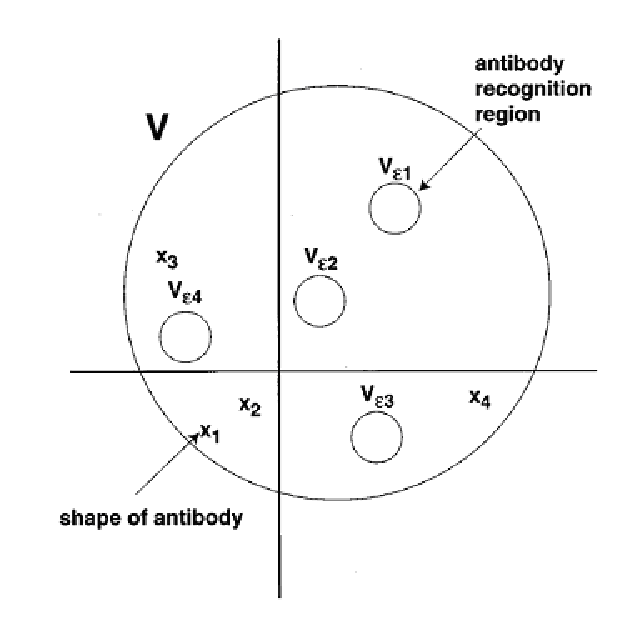
\includegraphics[scale=0.65]{ClonalSelection/theory-shapespace}}
	\caption{Depiction of the shape-space formalism taken from \cite{Perelson1997} (page 1225). $X_{i}$ represents antibodies with corresponding complementary recognition volumes $V_{\epsilon i}$.}
	\label{pic:theory:shapespace}
\end{figure}

%others
The shape-space formalism provides a geometric way to consider molecule interactions in the context of the immune system, it was not the first of such a geometric abstraction of molecular interaction. For example, Write considered a \emph{genotypic-space} for possible gene combinations and a mapping onto the now ubiquitous \emph{fitness landscape} in theoretical genetics \cite{Wright1932}. 
% usage
This fundamental $ag-ab$ interaction paradigm was used throughout the late 1980's and 1990's predominantly in theoretical works modelling clonal selection and various aspects of Jerne's idiotypic network theory (for example work on a one-dimensional Euclidean shape-space by Segel \cite{Segel1988}, and an investigating the stability of the idiotypic model by Perelson \cite{Perelson1989}). Carneiro and Stewart criticised the shape-space formalism, focusing on the simplicity of the abstracted space and the shortcomings of the simple affinity functions \cite{Carneiro1994}. They cautioned against the extrapolation of results from the abstraction to the real shape-space, highlighting that the dimensionality of the space should be much higher (at least 10, and as high as 20), and that the affinity mapping function would have to be irregular and discontinuous. They support their claims with observations from simulated docking of molecules based on crystallographic structures. They propose a splitting of the formalism into a \emph{realistic shape-space} in which real molecules can be evaluated, and an abstracted \emph{inversion space} as a tool for modelling.

%
% Affinity Landscape
%
\subsubsection{Affinity Landscape}
\label{subsubsec:cs:theory:affinitylandscape}
It is typical in physics for systems to minimise some utility in the context of a response surface, whereas in biology it is common for systems to maximise some utility. This is highlighted by the already mentioned evolutionary fitness landscape paradigm introduced by Wright in conceptualising gene combinations \cite{Wright1932}. In the immune system, one may consider the utility of an antibody as its affinity in binding to a specific antigen. A related concern called \emph{avidity}, refers to strength of the binding between antigen and antibody. Among the first to employ the conceptualisation of an \emph{affinity landscape} were Kauffman and Weinberger who used this geometric paradigm in the field of theoretical immunology to investigate and describe the theoretical effects of affinity maturation \cite{Kauffman1989, Kauffman1988}. They investigated adaptive walks using Kauffman's NK\footnote{Not to be confused with Natural Killer cells, $N$ and $K$ are parameters of the Kauffman's model.} model on the affinity landscape based on antibody sequences or so called \emph{antibody-space} in response to a given antigen. Kauffman and others used the NK model to investigate various molecular sequence spaces and the corresponding response surfaces, for example \cite{Farmer1986, Kauffman1993, Kauffman1987}. One may define an affinity landscape as a degree of complementarity response surface for a given collection of antigen detecting agents (lymphocytes and antibody), for a given \emph{specific} antigenic determinant. Abstractions of this surface considered in theoretical immunological are typically continuous, the topology of which consists of many local optima. Detecting agents may navigate this response surface through the process of affinity maturation, which involves manipulations to genotypic sequence information (such as the clonal selection diversity mechanisms discussed in Section~\ref{subsubsec:theory:diversity}).

The affinity landscape is a simple yet important conception, and although Kauffman et~al. were perhaps the first to apply such a name, the geometric formalism was no doubt in the mind of Perelson and others in the early days of theoretical and computational immunology. The formalism has played an important role in conceptualising and formalising \emph{affinity maturation} of the immune response by hypermutation (for example see \cite{Pierre1997, Shannon1999, Theodosopoulos2004, Theodosopoulos2005}), which as has been demonstrated is a critical aspect of the clonal selection theory of antibody diversity. George and Gray used the affinity landscape as a crutch in describing their theories on receptor editing, which were generalised very effectively on a simple two-dimensional affinity graph in Figure~\ref{pic:theory:affinitylandscape} \cite{George1999, George2000}.

\begin{figure}[ht]
	\centering
	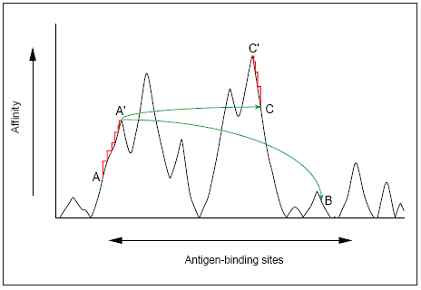
\includegraphics[scale=0.65]{ClonalSelection/theory-affinitylandscape}
	\caption{Theory of receptor editing providing long jumps in the affinity landscape, from \cite{George1999}.}
	\label{pic:theory:affinitylandscape}
\end{figure}

%
% Artificial Immune Systems
%
\subsubsection{Artificial Immune Systems}
\label{subsubsec:cs:theory:ais}
The shape-space and affinity landscape paradigms have been widely used in the field of Artificial Immune Systems. Some examples include the quintessential binary shape-space used in negative selection (for example \cite{Stibor2005}) and immune network algorithms, the recognition region and threshold used in data mining and classification algorithms \cite{Watkins2001, Watkins2004a, Knight2005}, and the affinity landscape cost functions navigated by optimisation algorithms \cite{White2003, Castro2002}. The usage of these paradigms is unified in the framework for AIS of Engineering de~Castro and Timmis, and listed in Section~\ref{subsec:background:problems:review}. The authors presented abstract models of immune cells, molecules and their interactions including the affinity landscape and shape-space paradigms in an effort to elaborate the three facets of their framework (representation, affinity measures, and immune algorithms). One may distil the discussion of the AIS Engineering Framework and related abstraction by de~Castro and Timmis, to a triad relationship between \emph{representation} in a shape-space, a \emph{mapping} function between points in that space, and an \emph{affinity landscape} of scores assigned by the mapping function, as follows:

\begin{itemize}
	\item \emph{Representation}: Extending the shape-space paradigm, the sequence, or search space is considered essentially a representation domain. Examples provided include real-valued, binary, integer and symbolic. 	
	\item \emph{Mapping}: A function that translates from the representation shape-space to an affinity landscape surface. Distance and matching within the shape-space are the mapping functions discussed with a number of appropriate suggestions for the various shape-spaces listed. A point in one of these spaces may have a \emph{recognition region}, and a \emph{cross-reactive threshold}. A mapping function may be complemented with an additional threshold binding function, perhaps to convert a scalar affinity into a decision variable.	
	\item \emph{Affinity}: Affinity may be further abstracted from the degree of complementarity in an antibody-antigen interaction, to a more general scoring assigned to the mapping between points in the shape-space. Affinity may be a measure of quality of an agent in a specific environment or in the context of a specific requirement.
\end{itemize}

The proposed triad provides a geometric interpretation and relation of \emph{shape-space} to \emph{affinity landscape} paradigms and provides an open framework for investigating immunological principles in domains, not limited to the pattern recognition problem. One may consider further geometric conceptions related to affinity maturation in immune system that lack a suitable formalism, let alone an abstraction for use in Artificial Immune Systems. Two examples may include: (1) the aggregation of multiple affinity landscapes, that is the affinity of a repertoire in the context of an antigenic environment not limited to one antigen, and (2) the temporal and spatial aspects to affinity throughout the host organism in the context of lymphocyte and antibody mobility.


%
% Clonal Selection Algorithms
%
\section{Clonal Selection Algorithms}
\label{sec:cs:algorithms}
The previous section outlined in detail the abstraction, immunochemistry, and theoretical immunology that inspired the field of clonal selection algorithms. The review highlighted that the main actors in clonal selection are cells, antibodies, and antigen, and the main processes are selection, proliferation, and genetic mutations. Further, it showed that the common measures used to describe the relationship between antibody and antigen are affinity and avidity, and that the main conceptual formalisms used to describe the constraints and effects of such interactions are shape-space and the affinity landscape. This section reviews the so called \emph{clonal selection principle} which is the abstraction that motivates the field of clonal selection algorithms. A taxonomy of such algorithms is presented, highlighting the open problems in the state of the art.

%
% From Theory to Principle
%
\subsection{From Theory to Principle}
\label{subsec:cs:algorithms:principle}
% de~Castro and Timmis
In the glossary of their seminal book on Artificial Immune Systems, de~Castro and Timmis provided a definition of the clonal `selection principle' as ``\emph{the prevalent theory stating that the specificity and diversity of an immune response are the result of selection by antigen of specifically reactive clones from a large repertoire of preformed lymphocytes, each with individual specificities}'', not distinguishing between the theory and information processing abstraction \cite{Castro2002a} (page 322). In their treatment of Burnet's theory, the authors comment that lymphocytes may be considered to undergo a process similar to natural selection and that only those cells that contact an antigen may be selected for proliferation, strongly highlighting the Darwinian connection made by Jerne and Burnet. The authors focused on the clonal expansion and variation aspects of the process, referring to the abstraction of the theory as \textbf{affinity maturation of the immune response}. They propose two important computational features of the theory in their abstraction (page 80): (1) An antigen selects multiple cells to proliferate where each cell has an individual clonal expansion rate proportional to its affinity to the antigen (\emph{higher affinity equals more clones}), and (2) the mutation of each cell during clonal expansion is inversely proportional to the affinity of cell to the antigen (\emph{higher affinity equals less point mutations}). The affinity proportional rates imposed on clonal expansion and mutation in their general clonal selection abstraction may be traced back to an earlier work of de~Castro and Von~Zuben on the seminal clonal selection algorithm CLONALG \cite{Castro2000} (discussed in Section~\ref{subsubsec:cs:taxonomy:clonalg}), in which they cited the work of Berek and Ziegner \cite{Berek1993}, commenting that a controlled cloning and mutation process could improve the efficiency of the process, and \emph{may} be employed by the immune system. 

% Cutello and Nicosia
In their treatment of the clonal selection and inspired algorithms Cutello and Nicosia proposed that clonal selection allows ``\emph{the learning of patterns during the primary response, and retrieval of previous knowledge during the secondary response or the cross-reactivity process}''  \cite{Cutello2005b} (page 112). They defined the abstraction of the theory called the \textbf{clonal selection principle} as involving both a learning or training phase followed by an applied or testing phase that may continue for the lifetime of the system, an approach which is common to the field of machine learning and pattern recognition. They proposed two key features of the clonal selection theory be taken into account in realising such a principle: (1) the \emph{hypermutation mechanism} which they consider a local search procedure that leads to a fast maturation during the learning phase, and (2) \emph{clonal expansion mechanism} that triggers the growth of a new population of high-value (affinity) cells. They consider all algorithms based on the clonal selection principle to be population based, where each member of the population represents a candidate solution belonging to the combinatorial fitness landscape of a given computational problem.

% my summation
What is distinctly common between these two sets of principles is (1) the absence of concerns of cell and antibody preparation for the task of pathogen identification associated with the negative selection paradigm, and (2) the absence of the concerns of cell-cell (inter-repertoire) interactions such as those associated with the immune network paradigm. Neither sets of principles explicitly exclude these concerns, rather they are not the focus of the information processing. The Cutello-Nicosia and the de~Castro-Timmis abstractions of the clonal selection theory are the two main sets of principles inspiring the IA and CLONALG families of clonal selection algorithms respectively (Section~\ref{subsec:cs:algorithms:taxonomy}). Both abstractions consider clonal selection to be an \textbf{adaptive process} that operates on a finite set of discrete units, the composition of which is changed though the iterative application of selection and clonal expansion with variation. Both abstractions also value the diversity provided through bind mutation that results in pre-committed configurations, some of which offer a relative selective advantage. The Cutello-Nicosia abstraction considers distinct training (change) and test (fixed) phases of adaptation, whereas the de~Castro-Timmis abstraction considers affinity-biased controls on a single adaptive phase. 

%
% Algorithm Taxonomy
%
\subsection{Algorithm Taxonomy}
\label{subsec:cs:algorithms:taxonomy}
This section presents a taxonomy of clonal selection algorithms that divides the scope of such algorithms into a genealogical tree of five groups, with a sixth miscellaneous group\footnote{This is the scope of clonal selection algorithms to the author's knowledge. It is not expected to be complete given the vastness and disparate nature of related publications, nor is it required to be complete for the purposes of this dissertation.}. The presented taxonomy only considers those algorithms that explicitly exploit (or claim to exploit) the clonal selection principle, which as outlined above requires the integration of the abstract actors and processes of the the clonal selection theory. Also listed in the miscellaneous category are examples of those AIS that although do not fit the adopted definition of a clonal selection algorithm, exploit considerable aspects of the clonal selection principle. Each linage is reviewed with regard to the core principles, exemplar algorithms, and summary of general application. Table~\ref{tab:cs:algorithms:taxonomy} provides a summary of each lineage and classified algorithms.

\begin{table}[ht]
	\centering\small
		\begin{tabularx}{\textwidth}{lXl}
		\toprule
		\textbf{Lineage} & \textbf{Algorithms} & \textbf{Primary Application} \\ 
		\toprule
		\emph{CLONALG} & CSA, CLONALG, CLONALG (1,2), ACS, CLONCLAS, RCSA, MOCSA, IMCSA, AISMM, SACSA, ECA & Optimisation \\ 
		\midrule
		\emph{AIRS} & AIRS, AIRS2, Parallel AIRS & Classification \\ 
		\midrule
		\emph{BCA} & BCA & Optimisation \\ 
		\midrule
		\emph{IA} & IA, SIA, I-PAES, CLIGA, CLIGA+, NC-IA, READ-Alg, opt-IA, opt-IMMALG, Par-IA, Dyn-IMMALG & Optimisation \\ 
		\midrule
		\emph{MISA} & MISA & Multi-Objective Optimisation \\ 
		\midrule
		\emph{Other} & Too large and varied to classify & Varied \\ 
		\bottomrule
		\end{tabularx}	
	\caption{Clonal selection algorithm taxonomy overview.}
	\label{tab:cs:algorithms:taxonomy}
\end{table}

%
% CLONALG
%
\subsubsection{CLONALG}
\label{subsubsec:cs:taxonomy:clonalg}
Hidden at the back of a technical report surveying the applications of Artificial Immune Systems, de~Castro and Von~Zuben  proposed the Clonal Selection Algorithm (CSA) as a computational realisation of the clonal selection principle for pattern matching and optimisation \cite{Castro1999}. This algorithm which has become perhaps the most popular in the field of AIS, was later published and represented \cite{Castro2000}, and again \cite{Castro2002} where it was renamed to CLONALG (CLONal selection ALGorithm). The general CLONALG model involves the selection of antibodies (candidate solutions) based on affinity either by matching against an antigen pattern or via evaluation of a pattern by a cost function. Selected antibodies are subjected to cloning proportional to affinity, and the hypermutation of clones inversely-proportional to clone affinity. The resultant clonal-set competes with the existent antibody population for membership in the next generation. In addition, low-affinity population members are replaced by randomly generated antibodies. The pattern recognition variation of the algorithm includes the maintenance of a memory solution set which in its entirety represents a solution to the problem. A binary-encoding scheme is employed for the binary-pattern recognition and continuous function optimisation examples, and an integer permutation scheme is employed for the Travelling Salesman Problem (TSP). Table~\ref{tab:cs:algorithms:clonalgparameters} summarises the algorithms parameters, and Algorithm \ref{alg:cs:algorithms:clonalg} presents a general formulation of the CLONALG.

\begin{table}[ht]
	\centering\small
		\begin{tabularx}{\textwidth}{lX}
		\toprule
		\textbf{Parameter} & \textbf{Description} \\ 
		\toprule
		\emph{P} & Repertoire of antibodies. \\ 
		\midrule
		\emph{N} & The fixed antibody repertoire size. \\ 
		\midrule
		\emph{n} & The number of antibodies to select for cloning. \\ 
		\midrule
		\emph{L} & Bitstring length for each antibody. \\ 
		\midrule
		$N_c$ & Number of clones created by each selected antibody. Originally expressed as a function of the repertoire size (for optimisation) $N_c=round(\beta \cdot N)$ (where $\beta$ is a user parameter), although a direct integer specification of $N_c$ is simpler. A rank-based (affinity proportionate) variation of the parameter is presented for pattern recognition. \\ 
		\midrule
		\emph{d} & Number of random antibodies to insert at the end of each generation. Random antibodies replace the $d$ lowest affinity antibodies in the repertoire. \\ 
		\midrule
		\emph{Stop condition} & Typically a specified number of generations or function evaluations or epochs of exposure to patterns. \\ 
		\midrule
		\emph{affinity} & Solution evaluation, typically the solution is decoded into a domain specific representation and assigned a quality scoring.  \\ 
		\midrule
		\emph{clone} & Duplication of a bitstring.  \\ 
		\midrule
		\emph{hypermutate} & Modification of a bit string where the flipping of a bit is governed by an affinity proportionate probability distribution. Originally $p=exp(-\rho \cdot f)$, although the opt-aiNET variant is also popular $p=(\frac{1}{\rho}) \cdot exp(-f)$ (where $\rho$ is a user parameter and $f$ is the normalised affinity scoring).  \\ 
		\midrule
		\emph{replace} & The set of the $d$ lowest affinity clones in the population ($P$) are replaced with randomly generated solutions. \\
		\bottomrule
		\end{tabularx}		
	\caption{CLONALG parameters.}
	\label{tab:cs:algorithms:clonalgparameters}
\end{table}

% CLONALG algorithm
\begin{algorithm}[ht]
  \SetLine  
  
  \SetKwData{Pop}{P}
  \SetKwData{Length}{L}
  \SetKwData{Selectsize}{n}
  \SetKwData{PopSize}{N}
  \SetKwData{RandomCells}{d}
  \SetKwFunction{StopCondition}{StopCondition}
  \SetKwFunction{Hypermutate}{Hypermutate}
  \SetKwFunction{Affinity}{Affinity}
  \SetKwFunction{Select}{Select}
  \SetKwFunction{Clone}{Clone}
  \SetKwFunction{Replace}{Replace}
  \SetKwFunction{CreateRandomCells}{CreateRandomCells}  
  
  \KwIn{\PopSize, \Selectsize, \Length, \RandomCells, $\beta$, $\rho$}		
  \KwOut{\Pop}
  
  % create cells	
	\Pop $\leftarrow$ \CreateRandomCells{\PopSize, \Length}\;
	
	\While{$\neg$\StopCondition{}}
	{
	 \ForEach{$p_i \in$ \Pop}		%// presentation
	 {
	 	\Affinity{$p_i$}\;
	 }
	 $P_{select} \leftarrow$ \Select{\Pop, \Selectsize}\;		%// clonal selection
	 $P_{clones} \leftarrow$ 0\;
	 \ForEach{$p_i \in P_{select}$}	%	// clonal expansion
	 {
	 	$P_{clones} \leftarrow$ \Clone{$p_i$, $\beta$}\;
	 }	 
	 \ForEach{$p_i \in P_{clones}$}		%// affinity maturation
	 {
    \Hypermutate{$p_i$, $\rho$}\;
	  \Affinity{$p_i$}\;
	 }	 
	\Pop $\leftarrow$ \Select{\Pop, $P_{clones}$, \PopSize}\;		%// greedy selection
	$P_{rand} \leftarrow$ \CreateRandomCells{\RandomCells, \Length}\;
	\Replace{\Pop, $P_{rand}$}\;	%// random replacement
	}
	\Return{\Pop}\;
	
	\caption{CLONALG for Function Optimisation.}
	\label{alg:cs:algorithms:clonalg}
\end{algorithm}


The work by Watkins, et~al was proposed to exploit the \emph{inherent distributedness} of the CLONALG \cite{Watkins2003}, as discussed in Section~\ref{subsec:distrb:review}. In the work, the pattern recognition variation of the CLONALG was modified such that each memory cell is partitioned to different processes and evolved independently or in small groups, the results from which are collated at the end of the algorithm run and returned as the algorithm result. White and Garret also investigated the pattern recognition version of CLONALG and generalised the approach for the task of binary pattern classification renaming it Clonal Classification (CLONCLAS) where their approach was compared to a number of simple Hamming distance based heuristics \cite{White2003}. Walker and Garrett investigated CLONALG and Evolution Strategies (ES) on dynamic function optimisation, showing that although CLONALG can achieve better results faster than ES on low dimensional dynamic functions, ES consistently outperforms CLONALG on the two high-dimensional problems tested \cite{Walker2003}. In an attempt to address concerns of algorithm efficiency, parameterisation, and representation selection for continuous function optimisation Garrett proposed an updated version of CLONALG called Adaptive Clonal Selection (ACS). The mutation parameter, the number of antibodies selected for cloning, and the number of clones produced for each antibody were changed to automatic parameters, controlled in a similar way to those in ES  \cite{Garrett2004}.
% many others
CLONALG is perhaps the most popular basis for elaboration and application with regard to clonal selection algorithms, specifically for function optimisation problem instances, the extent of which is excluded in the interest of brevity.

%
% AIRS
%
\subsubsection{Artificial Immune Recognition System}
\label{subsubsec:cs:taxonomy:airs}
After CLONALG, the Artificial Immune Recognition System (AIRS) algorithm is perhaps the second most popular clonal selection algorithm, although the approach was designed for and has only been applied to the supervised classification problem domains. The earliest work on AIRS was in Watkins Masters work \cite{Watkins2001} that was later published \cite{Watkins2002a}. The approach is a supervised learning algorithm for classification that uses the idea of an Artificial Recognition Ball (ARB) (introduced in earlier works on the Artificial Immune Network algorithm) to represent clones (groups) of identical B-cells. The AIRS procedure involves cloning and somatic hypermutation for preparing a set of real-valued exemplar vectors suitable for classifying unobserved cases, using a single iteration (epoch is the machine learning term) over a set of training data. Watkins and Boggess applied the AIRS to a suite of benchmark classification problems \cite{Watkins2002}, and Goodman and Boggess problems did the same, comparing to a conceptually similar approach called Learning Vector Quantization (LVQ) \cite{Goodman2002}.

Given the rapid popularity of the approach Marwah and Boggess investigated the algorithm seeking issues that affect the algorithms performance \cite{Marwah2002}. They compared various variations of the algorithm with modified resource allocation schemes, tie-handling within the ARB pool, and ARB pool organisation. AIRS was again raced against LVQ by Boggess and Hamaker on datasets that contained irrelevant features to assess the algorithms ability to handle noise \cite{Boggess2003}. Greensmith and Cayzer applied AIRS to hierarchical document classification \cite{Greensmith2003}, that culminated in Greensmith's masters work \cite{Greensmith2003a}. Watkins and Timmis proposed a new version of the algorithm called AIRS2 which became the replacement for AIRS1 \cite{Watkins2002b}. The updates reduced the complexity of the approach while maintaining the accuracy of the results. An investigation by Goodman, et~al. into the so called `\emph{source of power}' in AIRS indicated that perhaps the memory cell maintenance procedures played an important role \cite{Goodman2003}. A follow-up empirical investigation by Goodman and Boggess supported the original finding indicating that the process by which new memory cells are admitted into the ARB pool is critical to the success of the approach \cite{Goodman2004}.
% more
The work by Watkins, et~al., already mentioned briefly in Section~\ref{subsec:distrb:review} proposed a parallel version of AIRS permitting the division of training patterns and memory pool suitable to exploit parallel hardware \cite{Watkins2004}. The extent of further elaborations and applications of the approach are excluded in the interest of brevity.

%
% B-cell algorithm
%
\subsubsection{B-Cell Algorithm}
\label{subsubsec:cs:taxonomy:bca}
Kelsey and Timmis proposed the B-Cell Algorithm (BCA) as an AIS designed for continuous function optimisation \cite{Kelsey2003}. The algorithm maintains a pool of B-cells (binary-encoded candidate solutions) that are subjected to cloning and mutation. An elitist replacement population maintenance scheme is applied that ensures only improved cells are admitted into the pool. The mutation operator, which is called \emph{contiguous somatic hypermutation} selects a random sub-string of a solution to vary in a probabilistic manner, in what the authors claim as `hot-spot' mutation. Kelsey, et~al. applied the BCA to multi-modal dynamic chaotic test functions \cite{Kelsey2003a}. Empirical algorithm tuning by the authors revealed that small population sizes (3-5) show better results. In an investigation of AIS applied to optimisation, Hone and Kelsey provide a case study investigation of the BCA and showed fractal structures on the complex plane suggesting the potential usefulness of studying AIS as non-linear dynamical systems \cite{Hone2004}. In a further empirical study, Timmis, et~al. compared the BCA to opt-aiNET\footnote{(opt-aiNET) is an immune network algorithm for optimisation specified in \cite{Castro2002c}} and a Hybrid Genetic Algorithm attributing the partial success of BCA to the mutation scheme, speculating it results in the escaping of local-optima search behaviour \cite{Timmis2004a}. The parameters of BCA are summarised in Table~\ref{tab:cs:algorithms:bcaparameters}, and the general procedure for the approach is listed in Algorithm \ref{alg:cs:algorithms:bca}.

\begin{table}[ht]
	\centering\small
		\begin{tabularx}{\textwidth}{lX}
		\toprule
		\textbf{Parameter} & \textbf{Description} \\ 
		\toprule
		\emph{P} & Repertoire of antibodies. \\ 
		\midrule
		\emph{N} & Antibody population size. \\ 
		\midrule
		$N_c$ & Number of clones to create of each antibody. \\ 
		\midrule
		$N_r$ & Number of random antibodies to create and insert each generation. \\ 
		\midrule
		\emph{Stop Condition} & Typically if no progress is made for a number of generations. \\ 
		\midrule
		\emph{hypermutation} & Uses a processes called contiguous hypermutation, a random location in the bit string is selected, and a random bitstring length is selected. Each bit in the sub-string is flipped with the probability $\rho$. \\ 
		\midrule
		\emph{replace} & A parent is replaced only if a member of its clone has a higher affinity (greedy replacement). \\ 
		\bottomrule
		\end{tabularx}
	\caption{BCA parameters.}
	\label{tab:cs:algorithms:bcaparameters}
\end{table}


\begin{algorithm}[ht]
  \SetLine
  
  \SetKwData{Pop}{P}
  \SetKwData{Length}{L}
  \SetKwData{PopSize}{N}
  
  \SetKwFunction{StopCondition}{StopCondition}
  \SetKwFunction{Hypermutate}{Hypermutate}
  \SetKwFunction{Affinity}{Affinity}
  \SetKwFunction{SelectBest}{SelectBest}
  \SetKwFunction{Clone}{Clone}
  \SetKwFunction{CreateRandomCells}{CreateRandomCells}  
  
  \KwIn{\PopSize, $N_c$, $N_r$, $\rho$, \Length}		
  \KwOut{\Pop}      
  
  \Pop $\leftarrow$ \CreateRandomCells{\PopSize, \Length}\;
  
	\While{$\neg$\StopCondition{}}
	{
		\ForEach{$p_i \in$ \Pop} 		%// presentation
		{
	  	\Affinity{$p_i$}\;
		}	 
	 	\ForEach{$p_i \in$ \Pop}		%// clonal expansion
	  {
	  	$P_{clones} \leftarrow $ \Clone{$p_i$, $N_c$}\;	
	  	$P_{clones} \leftarrow $ \CreateRandomCells{$N_r$, \Length}\;	 %// random insertion
	  	
	  	\ForEach{$p_i \in P_{clones}$}		%// affinity maturation
	  	{
	   		\Hypermutate{$p_i$, $\rho$}\;
	   		\Affinity{$p_i$}\;
	   	}
	  	${p_i}\prime \leftarrow$ \SelectBest{$P_{clones}$}\;	  	
	  	\If{${p_i}\prime$.affinity $\leq$ $p_i$.affinity}
	  	{
	  		$p_i \leftarrow {p_i}\prime$\;
	  	}
	 	}	
	}
	\Return{\Pop}\;
	
	\caption{B-Cell Algorithm (BCA).}
	\label{alg:cs:algorithms:bca}
\end{algorithm}

A proof of convergence for the BCA was proposed by Clark, et~al. using a Markov~Chain model \cite{Clark2005}. The proof simplifies the algorithm to an elitist search with a single population member suggesting that the members of the population can be treated independently given the lack of interaction during the optimisation procedure. Further, they speculate that the introduction of inter-solution interactions in the BCA will have a detrimental effect on results of a search. Finally, in an empirical study Bull, et~al. applied the BCA to what they refer to as less-smooth test problem instances (Diophantine equations) seeking empirical convergence heuristics \cite{Bull2006}. Four variants of the algorithm were compared: an approach that used an elitist selection mechanism to introduce inter-solution interactions, and three of what the authors refer to as \emph{mega-mutation} schemes that attempt to introduce further diversity into the search. These less-greedy modifications of the approach achieved a better final result compared to the classical BCA on the test functions chosen, perhaps suggesting the use of diversity introduction approaches in further BCA applications. 

%
% IA Family
%
\subsubsection{Immunological Algorithm Family}
\label{subsubsec::cs:taxonomy:ia}
A simple clonal selection inspired algorithm was proposed by Cutello and Nicosia called Immunological Algorithm (IA) \cite{Cutello2002a, Cutello2002}\footnote{The Immunological Algorithm (IA) is renamed and represented many times by its authors. Other names include Simple Immune Algorithm (SIA), Cloning Information Gain Aging (CLIGA), and Optimization Immune Algorithm (opt-IA, opt-IMMALG). This linage is named the IA family for simplicity.} later renamed to Simple Immunological Algorithm (SIA) \cite{Cutello2005b}. The algorithm maintains a population of B-cells that are exposed to a clonal expansion process each iteration. This expansion process involves the cloning of cells and the application of a hypermutation operator, and was demonstrated on the Minimum Hitting Set Problem (MHSP) and the 3-Satisifiability Problem (3-Sat). The SIA was extended and an applied to the Graph Colouring Problem (GCP) \cite{Cutello2003}. The extensions involved the introduction of a local-search procedure that operated upon each B-cell after the clonal expansion phase. In addition, rather than an elitist selection method of maintain the population size after each expansion, an aging operator was introduced for each B-cell. B-cells are probabilistic deleted from the population using an equation inspired by the biological literature. Two variations of the aging operator were applied, an elitist version that ensured the best B-cell's were not deleted, and a pure strategy that probabilistically deleted irrespective of the elitist concerns. A birthing operator was also added to `top-up' the population to the configured size, and an information gain (a stabilisation in the measure of information discovered by the algorithm) measure was used as the termination criteria for the algorithm. Given the enthusiastic renaming and tweaking of this family of approaches, the SIA (the simplest variation of the family) is presented in Table~\ref{tab:cs:algorithms:siaparameters} and Algorithm \ref{alg:cs:algorithms:sia}.

\begin{table}[ht]
	\centering\small
		\begin{tabularx}{\textwidth}{lX}
		\toprule
		\textbf{Parameter} & \textbf{Description} \\ 
		\toprule
		\emph{P} & Antibody population. \\ 
		\midrule
		\emph{L} & Length of binary string representation. \\ 
		\midrule
		\emph{d} & Population (repertoire) size. \\ 
		\midrule
		\emph{dup} & The number of clones created for each antibody. \\ 
		\midrule
		\emph{clone} & Duplication of the bitstring. \\ 
		\midrule
		\emph{hypermutation} & Probabilistic modification of a bit string (bit flipping), requires the specification ($\rho$) of the probability of flipping each bit. \\ 
		\bottomrule
		\end{tabularx}
	\caption{SIA parameters.}
	\label{tab:cs:algorithms:siaparameters}
\end{table}


\begin{algorithm}[ht]
  \SetLine
  \SetKwData{Pop}{P}
  \SetKwData{Length}{L}
  \SetKwData{PopSize}{d}
  \SetKwData{CloneSize}{dup}
  
  \SetKwFunction{StopCondition}{StopCondition}
  \SetKwFunction{Hypermutate}{Hypermutate}
  \SetKwFunction{Affinity}{Affinity}
  \SetKwFunction{SelectBest}{SelectBest}
  \SetKwFunction{Clone}{Clone}
  \SetKwFunction{CreateRandomCells}{CreateRandomCells}  
  
  \KwIn{\PopSize, \CloneSize, $\rho$, \Length}		
  \KwOut{\Pop}    
  
  \Pop $\leftarrow$ \CreateRandomCells{\PopSize, \Length}\;
  
	\ForEach{$p_i \in$ \Pop}
	{
		\Affinity{$p_i$}\;		% // presentation
	}
	\While{$\neg$\StopCondition{}}
	{
		$P_{clones} \leftarrow$ 0\;
		\ForEach{$p_i \in$ \Pop}	% // clonal expansion
		{
			$P_{clones} \leftarrow$ \Clone{$p_i$, \CloneSize}\;
		}
		\ForEach{$p_i \in P_{clones}$}	% // affinity maturation
		{
			\Hypermutate{$p_i$, $\rho$}\;
			\Affinity{$p_i$}\; % // presentation
		}
		\Pop $\leftarrow$ \SelectBest{\Pop, $P_{clones}$, \PopSize}		% // clonal selection
	}
	\Return{\Pop}\;	
	\caption{Simple Immune Algorithm (SIA).}
	\label{alg:cs:algorithms:sia}
\end{algorithm}

The probabilistic aging operator was replaced with a simplified generational aging operator by Cutello, et~al. in an application to the 2DHP protein folding problem \cite{Cutello2004a}. In a more detailed study on different varieties of the same protein folding domain, the aging operator was further tweaked to facilitate longer life spans on some B-cells deemed useful to the search process \cite{Cutello2006b}. The clonal expansion aspect of the algorithm (cloning and hypermutation) was grafted into to an existing evolutionary multiple-object optimisation technique and called I-PAES \cite{Cutello2006a} . The transformed algorithm (generational aging, information gain stopping criteria) was reviewed and renamed to the `Cloning, Information Gain, Aging' (CLIGA) algorithm \cite{Cutello2005b}. A modified version called CLIGA+ was proposed in which each B-cell contains more than one receptor (pattern), permitting application of the algorithm to pattern recognition tasks. Also proposed in this work is a Noisy Channel variation of SIA (NC-IA), and a Reaction-Diffusion variation of SIA (READI-Alg) both of which were applied to instances of the GCP.  
% more
Cutello, et~al. again renamed the approach to Optimisation Immunological Algorithm (opt-IA) and applied the approach to instances of binary trap functions \cite{Cutello2004}. An additional fitness inversely-proportional hypermutation referred to as \emph{hypermacromutation} was proposed and compared to the traditional static approach. This algorithm was evaluated again in a larger study involving a number of machine learning domains \cite{Cutello2005a}, and again on a large number of continuous function optimisation instances \cite{Cutello2005c}. Cutello, et~al. investigated the hypermutation operators of opt-IA \cite{Cutello2004b}. Cutello, et~al. applied opt-IA to the 3DHP protein folding problem \cite{Cutello2005}. Cutello and Nicosia  applied opt-IA to graph colouring, MHSP, and satisfiability \cite{Cutello2006e}. Work by Anile, et~al. hybridised opt-IA with a direct search method \cite{Anile2006}. An extension of opt-IA called \emph{Aligner} was proposed by Cutello, et~al. and applied to multiple sequence alignment of DNA  \cite{Cutello2006}.

An extension to opt-IA was proposed by Cutello, et~al. called the parallel immune algorithm (Par-IA) which is a master-slave version of the algorithm applied to numerical function optimisation \cite{Cutello2006d}. Cutello, et~al. renamed the approach to Optimisation Immune Algorithm (Opt-IMMALG), applying the approach to continuous function optimisation using a real-valued representation as opposed to the binary representation used in previous works \cite{Cutello2006f}. Also stated in this work was the use of fitness inversely proportional hypermutation as the standard mutation operator for the approach. This algorithm was extended and renamed dynamic immune algorithm (dyn-IMMALG) by Cutello, et~al. who propose a dynamic rather than static clonal operator \cite{Cutello2006c}. The approach was applied to binary trap functions and compared to opt-IA and variations of CLONALG.

%
% MISA
%
\subsubsection{Multi-objective Immune System Algorithm}
\label{subsubsec:misa}
Coello~Coello and Cruz~Cortes introduced an AIS called the Multi-objective Immune System Algorithm (MISA), and as its name suggests was designed as a population-based approach for constrained and unconstrained multi-objective optimisation \cite{Coello2002}. In the approach a repertoire of solutions is split into antigens (Pareto non-dominated and feasible solutions) and antibodies (Pareto dominated and infeasible solutions). A bit-string representation is used and antigens are selected at random and matched against antibodies using Hamming distance. After the selection step, antibodies are cloned, mutated the population is unioned and reduced back to the configured size, culling the lower quality solutions. An external (elitist) memory repertoire is maintained of non-dominated feasible solutions. Solutions are added to the memory set if they are non-dominated by the current memory set population and sufficiently diverse as determined by a grid-based maintenance structure. MISA was extended by the same authors and further compared to state of the art evolutionary approaches for multi-objective optimisation \cite{Cortes2003}. An EC-AIS hybrid terminology was adopted and an EC-based crossover mechanism was adopted within the memory set. The main algorithm was simplified such that all population members were consider antibodies, and only the lower score solutions was selected for cloning and hypermutation. The modified algorithm was shown effective, although it demonstrated rapid convergence behaviours on benchmark problem instances. Finally, Villalobos-Arias, et~al. proposed a convergence proof for the update MISA showing that the elitism within the algorithm was needed to guarantee convergence  \cite{Villalobos-Arias2004}.

%
% Other
% (those do not easily fit into the taxonomy)
%
\subsubsection{Other}
\label{subsubsec::cs:taxonomy:other}
% all the works that do not fit the taxonomy
Research into the five core lineages of clonal selection algorithms revealed a large number (\textgreater70 works) on new or extended clonal selection algorithms, predominantly in non-western conference proceedings. The vast majority of these works involved the application of a CLONALG, SIA, or derivative algorithms to benchmark and engineering problem domains. The extent of these works are omitted here for brevity, although the dominant applications are listed as follows: feature selection for models, parameter tuning for models or controllers, parameter tuning for a PID controllers, anomaly and/or intrusion detection, pattern recognition, multi-objective optimisation, function optimisation, general optimisation, multi-user detection, and finally hybridisation with other algorithms.

% example AIS works that explicitly use clonal selection, but do not fit into the taxonomy
As discussed in Section~\ref{sec:background:threeschools}, the clonal selection principle underlies the adaptive qualities of all three of the major paradigms of Artificial Immune Systems. As such, many works investigating the negative selection and immune network employ B-cells and antibodies that are modified using processes of selection and expansion with variation. Given that these approaches do exploit the clonal selection principle they may be considered clonal selection algorithms, although do not fit into the presented taxonomy as the clonal selection principle is not the primary focus of the works. This section provides some examples of such research. Weinand propose a dynamical systems computational model of somatic mutation of B cells to evaluate the effect of somatic mutation of affinity maturation of the immune response \cite{Weinand1990}. Zhang and Hou propose a Niching Clonal Selection Algorithm (NCSA) that combines negative selection and refinement applied to the pattern matching problem of anomaly detection \cite{Zhang2003}. Yu and Hou proposed an extension of CLONALG called CsAL (Clonal Selection Algorithm) to investigate the negative selection approach to virus detection \cite{Yu2004}. In the body of work on an integrated intrusion detection system discussed in Section~\ref{subsec:distrb:review}, the authors propose a static and dynamic clonal selection algorithms (DynamiCS) which are an augmentation to T-cell inspired negative selection system that uses clonal selection mechanisms to improve detectors. 

%
% Criticisms and Open Problems
%
\subsection{Criticisms and Open Problems}
\label{subsec:cs:algorithms:problems}
% state of CSA is limited
The review of the clonal selection principle demonstrated that abstractions of the theory are generally simplistic, considering the information processing properties and mechanistic procedure at a high-level, correlating the general AIS observations made in Section~\ref{sec:background:openproblems}. 
% overview
The authors de~Castro and Timmis reduced clonal selection to a single antigen optimisation system using affinity maturation with controlled affinity-proportionate cloning and inversely affinity proportional mutation. Cutello and Nicosia reduced clonal selection to the more general life-long acquisition and retrieval for application of patterns. The common features to clonal selection abstractions are the properties of (1) population based information processing (2) clonal expansion of selected high affinity population members, and (3) affinity maturation via mutation of clones. The commonly executed concerns of the abstractions include (1) concerns of self and nonself discrimination (cell preparation), (2) distinction between cell types and/or antibody molecules, and (3) cell-cell interactions.

% existing approaches
The realised clonal selection algorithms are monolithic, considering antibody conformations in binary and real value shape-spaces, mostly against a single affinity landscape. As such, the dominant application domains are optimisation (function optimisation), and supervised classification with procedures that closely resemble genetic algorithms (CLONALG, IA, BCA, MISA) and vector quantisation procedures (AIRS), and the dominant conceptual and quantitative comparisons have been made with evolutionary algorithms. The review demonstrated that the trend with these approaches have been to (1) enhance the algorithm procedure through domain specific assumptions (limited resources in the case of ARB for classification, and affinity proportionate descent with modification in CLONALG for optimisation), (2) tweaking and parameter tuning (numerous additional and alternative operators in the IA family, sensitivity analysis of CLONALG, BCA and AIRS), and (3) application, benchmarking and racing (the majority of the published research).
% limitations
Based on the detailed review of the state of the art of clonal selection algorithms in the context of clonal selection and related theory, this section identifies three specific limitations that represent open problems in the field, as follows:

\begin{enumerate}
	% broader field
	\item \emph{Related Approaches}: Clonal Selection Algorithms have generally been related and compared to Evolutionary Algorithms including the Genetic Algorithm and the Evolutionary Strategy, although broader connections with related computational intelligence fields are typically brief and/or non existent. Systematically placing and contrasting Clonal Selection as a Computational Intelligence metaphor with related paradigms provides both a context for comparison of behaviour and capability, and suggests at the specific overlapping features and findings that may be exploited as well as those features that differentiate the approach and should be pursued.

	% adaptation
	\item \emph{Implicit Adaptive System}: Given the adaptive qualities of the clonal selection theory, computational models are implicitly assumed to be instances of adaptive systems. Whether or not a CSA is an adaptive system is not in question, rather the more important concerns of what it means for computational models of clonal selection to be classified as adaptive systems. Unlike the Genetic Algorithm that emerged from Holland's investigation and formalisation of adaptive systems, the inception and investigation of clonal selection algorithms has been focused on addressing benchmark instances of difficulty computational problems. The consideration of the clonal selection as a strategy in the context of an adaptive systems formalism will provide a stronger foundation of understanding, and insights into the broader and unrealised information processing capabilities of the approach.
	
	% beyond 
	\item \emph{Cellular Focus}: The scope of clonal selection algorithms are concerned with abstractions of lymphocyte interactions with antigen, specifically with little or not detail of the molecular basis of such interactions, nor the broader consideration of where such interactions occur or the effect they have on the host organism. This cellular focus is reasonable for the preliminary realisation of computational models inspired by the theory embodied in the present state of the field, although elaboration and development of so-called `second generation' clonal selection algorithms requires a holistic consideration of the acquired immune system and the restrictions and constraints such a broader perspective imposes on improvement-centric adaptive clonal selection strategies.
\end{enumerate}


%
% Summary
%
\subsection{Summary}
% general
The detailed treatment of the Clonal Selection Theory in Section~\ref{sec:cs:theory} provided the context for effectively appraising the state of clonal selection algorithms, specifically with regard to the task of identifying limitations which may be exploited toward elaborating the general approach.
% taxonomy
The taxonomy presented in Section~\ref{subsec:cs:algorithms:taxonomy} unified disparate works by general algorithm lineages, that ultimately highlighted both the deep commonality between the lineages and the algorithms that belong to them, and the simplicity of the overarching computational abstraction that underlies such approaches.
% limitations
Importantly this insight provided the context to identify three limitations and open problems with the clonal selection paradigm that motivate the remainder of this Chapter. Specifically, Section~\ref{sec:cs:related} reviews machine learning approaches to clonal selection highlighting the findings that may be exploited and the features that differentiate the approach. Section~\ref{sec:cs:adaptive} considers the clonal selection strategy in the context of adaptive systems theory, highlighting critical features of the theory excluded and underrated by existing computational abstractions. Finally, Section~\ref{sec:cs:beyond} address the cellular focus of the paradigm, and outlines an agenda for extending the approach beyond a discrete repertoire of cells toward distributed clonal selection algorithms.


%
% Related Computational Paradigms
%
\section{Related Computational Paradigms}
\label{sec:cs:related}
This section considers some related machine learning paradigms and their relationship with the clonal selection principle and inspired algorithms. This review includes both related paradigms that have been previously considered such as Evolutionary Computation and Reinforcement Learning, and additional newly considered paradigms such as Lazy Learning, Competitive Learning and Hill Climbing. The intent of this investigation is to highlight findings from related computational paradigms that may provide insight into the behaviour, function, and/or capability of the current state and potential elaborations of clonal selection algorithms.
% all pop the same
An interesting aside is the work by Newborough, et al. \cite{Newborough2005} provide a framework that suggested that all population algorithms (including clonal selection) may be treated in a similar manner.

%
% Evolutionary Computation
%
\subsection{Evolutionary Computation}
\label{subsec:cs:related:ec}
% overview
Evolutionary Computation (EC) is a field of study of Evolutionary Algorithms (EA's) that has much in common with AIS, although draws its inspiration for computation from \emph{Darwinian} (theory of natural selection) and \emph{neo-Darwinian} (findings of modern genetics also referred to as the new synthesis) theories of evolution. Clonal selection algorithms have a superficial similarity to some EC algorithms such as the Genetic Algorithm (GA), and to the properties of modern Evolution Strategies (ES). See \cite{Fogel1995, Goldberg1989a} for a classical treatment of EC and \cite{Back2000, Back2000a} for a modern treatment of the field of EC. 

% review
In their work on CLONALG, de~Castro and Von~Zuben consider the similarity between a GA and their approach, particularly in regard to the binary representation used and the stochastic-Darwinian processes employed by both algorithms \cite{Castro1999}. They suggest the differences between the algorithms, include the vocabulary used (genetics and evolution verses the shape-space formalism and antibody-antigen cellular interactions), and the somatic mutation and receptor editing used to explore the shape space. The authors also claim that CLONALG can be categorised as an \emph{evolutionary-like algorithm}, although they maintain the same arguments of inspiration, vocabulary, and formalism and the primary differences \cite{Castro2002}. In their book de~Castro and Timmis again acknowledge the similarity of CLONALG to an EA \cite{Castro2002a}. They are quick to point out that a major difference between the inspirations of the two approaches is that mutation in evolution is random, whereas the hypermutation process of clonal selection is controlled and directed, proportional to the receptors affinity with the triggering antigen (specific to their abstraction). They suggest that work on EA's can be leveraged by CSA's indicating that research on selection operators (e.g. tournament and roulette wheel selection) may be exploited. The shape-space formalism is presented as a CSA representation abstraction where non-binary shape-space schemes and corresponding mutation mechanisms are discussed, also leveraging from research from representation and mutation in EA's. The authors provide a treatment of evolution and the clonal selection of the acquired immune system. They suggest an important difference between the two theories is the fact that in the clonal process expansion occurs through cell cloning, that there is no sex or genetic recombination, rather only affinity inversely-proportionate somatic hypermuatation.

% more 
In work on the MISA, Coello~Coello and Cruz~Cortes claim that their approach is not a genetic algorithm because it does not use recombination (crossover operator) \cite{Coello2002}, they later adopt a crossover procedure in their approach, as well as adopt a hybrid of EC and AIS terminology \cite{Cortes2003}. In their work evaluating the BCA on function optimisation Timmis, et~al. suggest that BCA is not a GA, based on the empirical performance of the approach on a small suite of test problem instances, although they are very quick to point out the limitations of their small study and the requirement for further research \cite{Timmis2004a}. Forrest, et~al. investigated the pattern recognition properties of the immune system \cite{Forrest1993a}. They used a binary coded GA to model antibody-antigen matching in the immune system, which included the clonal selection mechanism, claiming ``\emph{The GA without crossover is a reasonable model of clonal selection, while the GA with crossover models genetic evolution}". Hightower, et~al. use a Binary GA model of somatic hypermutation of clonal selection to investigate the Baldwin Effect and evolution \cite{Hightower1995}. Fukuda, et~al. \cite{Fukuda1993} and Mori, et~al. \cite{Mori1993a} used a GA to investigate clonal selection properties and immune network algorithms for scheduling and resource allocation. The niching-like properties (an EA property inspired by theories of population genetics and ecology) were observed by de~Castro and Von~Zuben with CLONALG on multi-modal function optimisation \cite{Castro2002}, and empirically compared to the fitness sharing approach of Goldberg, et~al. \cite{Goldberg1989a, Goldberg1987, Deb1989}. The niching search properties were proposed to occur given the hill-climbing like behaviour of the independent and semi-independent evolution of B-cells of the various clonal selection algorithms. 

% similarities
The principle similarity between evolutionary algorithms like the genetic algorithm and clonal selection algorithms is the Darwinian inspired theories that inspire both fields (selection and descent with modification). Natural selection accounts for the diversity of species, whereas clonal selection accounts for the diversity of antibodies. As such, both processes are imperfect, stochastic process that operate on pre-committed discrete individuals with short terms goals (relative selective advantage). 

% differences
The differences between the sub-fields are subtle, related to the functional specifics of the inspired theories. The theory of natural selection encompasses that of clonal selection, as the genetics of the organism define the fitness of that organism, one aspect of which is the structural and function aspects of the organisms adaptive immune system. Related to this point is that of the time-scales involved, evolution of species such as mammals involves the accumulation of small changes over geological time, where as the accumulation of changes in clonal selection are exploited by a single host over its lifetime. Although in both cases selection, decent, and modification occur on genetic material, the hereditary of evolution is the entire genome, where as the hereditary of the B-cell lines are those genes which affect antibody structure. The time-scales also highlight the properties of learning within the host, evolution involves learning at the species level with a single host representing a pre-committed unit of adaptation, whereas acquired immunity involves learning within the host, like the learning that occurs within the brain, so called lifetime or meta-ontogenetic and meta-epigenetic (non-inheritable changes to DNA) adaptation. The differences go beyond nomenclature to the specifics of the inspired processes. Selection in the immune system as a discrete event that triggers (or does not trigger) an immune response resulting in decent with modification. Selection or survival of the fittest is an abstraction that involves relative differences in reproductive success not contingent on anticipated triggered events. The clonal expansion process involves mass replication via cell division where modification is introduced through high-probability point mutations in related genes. Darwinian evolution employs both sexual and asexual reproduction, although evolutionary algorithms typically exploit the crossover of genetic material and point mutations to introduce variation.

%
% Binary Hill Climbing
%
\subsection{Binary Hill Climbing}
\label{subsec:cs:related:hillclimbing}
% overview
A realisation of the clonal selection principle includes the choice of strings of bits as a first-order representation. This choice of representation is (1) amenable to analysis and (2) amenable to remapping, and (3) provides a genetic metaphor facilitating genetic-like operations such as copying errors during cell division. The use of binary strings as a first-order representation is pervasive in computational intelligence, particularly in the field of evolutionary computation. Section~\ref{subsec:cs:related:ec} demonstrated that there has been much consideration of the relationship between EC and CSA, although little attention has been given to strong relationship between optimisation-driven CSA's and binary hill climbing. This section considers this relationship by providing a brief overview of the state of the field.

% detail
The genetic adaptive plan which became the genetic algorithm operates on a population of bit-strings. This representation facilitated the genetic operators of the approach, and the analysis of the behaviour of the system as processing building blocks (schemata theorem). One of the generalised genetic operators is mutation, the probabilistic flipping of bits in the bitstring during genetic replication. Holland proposed that mutation is determined ``\emph{by a random process where each position has a small probability of undergoing  mutation, independently of what happens in other positions}" \cite{Holland1992} (page 109). In using random mutation alone Holland suggested the use of small mutation probabilities such that the process provides a high probability of maintaining history, which is the dependence of the approach. Holland pointed out the use of high mutation values results in little dependence between successive generations of individuals, calling such an approach \emph{essentially enumerative}. Low probability mutation facilitates the dependence between observations and new trials, although is suggested to be \emph{very unsophisticated} compared to genetic crossover. He proposed the use of low probability mutation as an improvement operator for existing solutions that rather than used in the construction of new trials. He proposed the operator should be used to complement the primary genetic operator by restoring lost genetic material. Further, the application of the mutation operator was described to be disrupting to the building blocks moved around by the crossover operator, further reinforcing the need for a low probability of occurrence. Holland called mutation a background operator, and thus the effects of the operator were largely ignored, and the probability of point-mutations was conventionally kept very small (for example $P_m \in  \left[0.001,0.01\right]$) \cite{Goldberg1989a, Back2000}. The probability of a bitstring being mutated is $P_m = 1 - (1-p_{m})^L$ where $P_m$ is the mutation rate and $L$ is the string length. Goldberg differentiated between mutation and crossover by suggesting that \emph{selection+mutation} provides continual improvement with limited scope, whereas \emph{selection+crossover} provides innovation via jumping and remixing of components \cite{Goldberg2002}. 

Eiben and Schippers summarised the role of the mutation operator as a uninary (or asexual) and unbiased operator, highlighting its role as a main operator in evolutionary strategies (traditionally real numbers) and the primary operator in evolution programming (traditionally operates on finite state machines) \cite{Eiben1998}. Spears highlighted the complementary nature of the two primary genetic algorithm operators suggesting that mutation the focus if optimality is important and the crossover is useful accumulated payoff is important \cite{Spears1992}. He suggested that crossover and mutation are two versions of the same general operator that perturbs genetic representations based on available information. In his dissertation, Spears proposes that mutation has a high exploratory power (in that it is not dependent on the composition of the population) and no positional dependence (in that it has the potential to transform a given string into any other string in the search space) \cite{Spears1998}. Work by Schaffer, et~al. in the late 1980's and early 1990's highlighted the potential of the mutation operator, suggesting the operators power had been underestimated in genetic algorithms \cite{Schaffer1991, Schaffer1989}. These works attempted to formalise an optimal mutation rate for genetic algorithms, work that was extended experimentally in \cite{Schaffer1989} and theoretically \cite{Hesser1991}. Later work suggested the use of an initially large mutation rate that exponentially decreased with generational running time of the algorithm. A dynamic and decreasing mutation rate was further supported by others investigating the potential of the operator (not  limited to \cite{Muhlenbein1992, Fogarty1989}). The reason for this is ``\emph{the probability that a mutation will give a better string decreases with the number of bits which are correct}" \cite{Back1993}.
% more
A simplified genetic algorithm was proposed for investigating the strengths and limitations of the mutation operator, which became known as a mutation hill-climber, (1+1,$m$) \cite{Muhlenbein1992} or simply (1+1) \cite{Back1993}. The algorithm has a static mutation probability ($P_{m}$) applied uniformly and independently to each bit in the bitstring. The algorithm was called a hill climber because without crossover, there is no inter-population interaction of genetic information, thus if a population is used, it is a collection of unrelated parallel hill climbers. The (1+1) is taken from the Evolution Strategy naming convention ES($\mu$+$\lambda$) where $\mu$  parents create $\lambda$ offspring, and the best from both `+' are selected. The scheme was reduced to a single parent and offspring for ease of analysis. The algorithm has the interesting property as a hill climber that there is no well-defined neighbourhood for a given string. Rather, a probabilistic neighbourhood is defined by the mutation probability. This neighbourhood covers the entire search space such that it is possible to move from a given string to any other string in the space, a probability that decreases with the increase in Hamming distance between strings and the current string. M{\"u}hlenbein analysed the algorithm and proposed an approximate optimal mutation rate (the standard mutation rate) as $P_{m} = \frac{1}{L}$.

% clonal selection
The CLONALG, BCA and the basis of the IA family (SIA for example) are elaborations of either a parallel Random Mutation Hill Climbing Algorithm (RMHCA) or the (1+1,m)-Algorithm. As such, it is reasonable to consider the state of (optimisation-based) clonal selection algorithms as investigations into parallel hill climbers (GA's without crossover as commented by Forrest, et~al. \cite{Forrest1993a}). A fair assessment of algorithms such as CLONALG, BCA, and the IA family requires the consideration of the decades of empirical and theoretical findings from this related field, such as mutation rates, test problems, and existing hill climbing and mutation-based hill climbing algorithms for comparison. This perspective may also highlight a severe weakness in the state of the art of optimisation-centric clonal selection algorithms.

%
% Lazy Learning
%
\subsection{Lazy Learning}
\label{subsec:cs:related:lazy}
% overview
Instance-based learning is a non-parametric and supervised machine-learning paradigm where a model is constructed from domain data instances at query time. The complexity increases with the quantity of data, and the more data available, the more specific the model \cite{Aha1991a, Russell1995}. Instance-based learning is typically referred to as Lazy Learning, which is a machine learning paradigm where generalisation occurs as required. Lazy learning may be contrasted with Eager Learning in which generalisation occurs before a query is received. In addition to the deferral of generalisation, lazy learning is also typified by the combination of stored data used to reply to requests, and the fact that the response is discarded after it is delivered \cite{Aha1997, Aha1998, Wettschereck1997}. The thee principle characteristics of lazy learning are: \emph{Defer}: Store all training data and defer processing until queries are given that require replies, \emph{Demand-Driven}: Queries are answered by combining training data, using a local learning (neighbourhood) approach. Instance are (1) identified in as points space, (2) a similarity measure is used to define the neighbourhood, (3) prediction function uses information to answer a query. \emph{Discard} the answer and any intermediate results after answering the query.

% detail
Instance-based learning may be considered a type of local learning algorithm, where reasoning is based on models (kernels) constructed from instances similar to the input instance. A typical concern with such models is the capability of the system to generalise. This represents a trade-off between the capacity (size) of the model and the number of samples to consider in the model. Bottou and Vapnik rephrased this local learning trade-off to be between the capacity of the model and the locality of the samples, where locality is the shape and size of the instance selection region (neighbourhood) \cite{Bottou1992}. This locality property of model construction defines how local an algorithm is, such that an instance-based approach such as $k$-Nearest Neighbour is highly-local with a low capacity, and a connectionist approach such as a neural network is non-local with high capacity. Case-based Reasoning (CBR) (or memory-based reasoning), is a generalised application of instance-based learning applied to reasoning such as expert systems \cite{Aha1991}. Aamodt and Plaza provide a concise description of the various different identities of instance based learning from a case-based reasoning perspective \cite{Aamodt1994}. Their taxonomy highlights the perspective each identity places on this style of learning which covers exemplar, instance, memory, case, and analogy based learning and reasoning. Further, Aamodt and Plaza propose a descriptive framework for CBR, which includes a general algorithmic cycle for the application of the approach, as follows: \emph{Retrieve} the most similar case or cases, \emph{Reuse} the information and knowledge retrieved to solve the problem, \emph{Revise} the proposed solution, and \emph{Retain} the parts of the experience that may be useful for future problem solving.

% more
There are two primary classes of lazy learning approaches: Nearest Neighbour Methods, and Kernel Methods. Nearest neighbour methods are function approximation algorithms that search through a database for similar instances (cases) to a given input instance and make a prediction \cite{Cover1967}.  The similar points to consider in the prediction are referred to as the neighbourhood, and the number of points is typically denoted $k$, thus the scheme may be referred to as $k$-nearest neighbour or $k$NN. A natural extension to nearest neighbour approaches is that each case generates a local density function or kernel. Predictions may be made by summing together densities functions. The kernel function depends upon the distance function between cases, where the Gaussian is a typical function employed. Some techniques include distance weighted regression such as Linear Weighted Regression methods \cite{Atkeson1997}, and a neural-network like approach called Radial Basis Function \cite{Broomhead1988, Buhmann2000, Powell1987}. Much of the work on instance based learning algorithms is focused on reduction of storage requirements (thus increasing the efficiency of the approach), and improving the algorithms robustness to with regard to attribute noise and irrelevant attributes. Perhaps the most popular concern of nearest neighbour based approaches is what has been referred to as the \emph{curse of dimensionality}. This refers to the fact that in common datasets, the nearest neighbour is approximately the same distance away from a given point as the furthest neighbour. This effect is observed in dimensions as low as 10-15 \cite{Beyer1998}. The problem is caused by the exponential increase in volume of a space by the adding of additional dimensions\footnote{It should be noted that the curse of dimensionality has been considered in the context of negative selection algorithms by Stibor, for example \cite{Stibor2006}}. 

% clonal selection
The clonal selection principle does share some commonality with the instance based learning, particularly in the context of the continual adaptation to antigen and Aamodt and Plaza's four R's of CBR. The specific knowledge about the antigen is discarded after the infection is addressed, although is retained implicitly in the selected cognate receptors. The AIRS is a realisation of clonal selection that considers the the repertoire as a model of cases that are compressed (quantised) to a set of exemplars. For example, a recent work by Seeker and Freitas \cite{Seeker2007} make the argument that AIRS is nothing more than an instance-creating algorithm for use by $k$NN. Exemplar-based modelling is used in a variety approaches for function approximation problems (such as the LVQ algorithm), which represent an important application perspective on clonal selection algorithms (considered further in Section~\ref{sec:iidle:function:approximation}). A similar approach was taken on the pattern recognition variation of CLONALG, although the number of patterns was known and not compressed as in the case of AIRS. 



%
% Competitive Learning
%
\subsection{Competitive Learning}
\label{subsec:cs:related:competitive}
% overview
Intrator and Edelman commented that competition between functional units is a widespread biological phenomenon, particularly in the vision systems, the brain, and other sensory systems \cite{Intrator1997}. Competitive learning systems are based on the idea of competition for activation, and lateral (same level) inhibition. Without inhibition, the models result in an averaged or muddied converged state. They define competitive learning as a dynamic redistribution of responsibilities of various units over parts of the representation space and propose a global, local, and a hierarchical perspective. The authors suggest that resource allocation may be addressed through selective inhibition, such that those units or modules that have not been activated for some time are inhibited less. Further, they suggest investigation into two types of competitive learning: (1) competitive learning via lateral inhibition, (2) competitive learning via the top-down separation of flows of information. Three perspectives of competitive learning are as follows \cite{Intrator1997}:

\begin{itemize}
	\item \emph{Global Competition} Competition over the entire representation space, with a strong requirement for inhibition via lateral connections between neurons and the distinction between hard (single winner) and soft (multiple winner) competition
	\item \emph{Local Competition} The division of the representation space such that local experts (modules of units) compete (known as mixture of experts). Assumes that different processes generate different parts of the representational space, thus hard competition assume a one-to-one matching between modules and hidden generator processes that they model.
	\item \emph{Hierarchical Competition} A mixture of global and local competition, where the representation space is partitions or split into a hierarchical tree structure.
\end{itemize} 

% detail
Competitive learning is a connectionist machine-learning paradigm where an input pattern is matched to the node with the most similar input weights, and the weights are adjusted to better resemble the input pattern. This is called the \emph{Winner-Take-All} (WTA or maximum activation) unsupervised learning method where the input pattern is compared to all nodes based on similarity. The nodes compete for selection (or stimulation) and ultimately adjustment (or learning) \cite{Luger1997}. Some popular competitive learning algorithms include Kohonen's Self-Organising Map (SOM), Adaptive Resonance Theory (ART), and Counterpropagation Networks, and Neural Gas. SOM is a seminal achievement in the field of competitive learning inspired by the spatial order and organisation of brain functions \cite{Kohonen2001}. The Self-Organizing Map is an unsupervised learning algorithm (clustering) that embodies the WTA principle and facilitates topological preservation in the face of dimensionality reduction. The Learning Vector Quantization (LVQ) is a supervised learning algorithm (classification) and is a zero-order SOM with no connectivity between nodes. Without the connectivity, there is no geometry or topological neighbourhood effects, although the unstructured collection of exemplars compete for stimulation using the winner-take-all principle, and winners that miss-classify during the training process are suppressed. A problem with the winner-take-all learning principle is that units may win too much, and thus dominate selection and response. The result is that some units may never win and the units are considered dead (resources are underutilised) \cite{Rumelhart1985}. A relatively simple solution is to dampen the competitiveness of the principle by keeping track of how often units win competitions and using this information to reduce the chance of wining in the future. This may be achieved by introducing a conscience to the units \cite{DeSieno1988}, or a similar method called frequency-sensitive competitive learning \cite{Ahalt1990}. This effect may also be achieved by using a generalised version of the suppression mechanism of LVQ2 called rival-penalised competitive learning, where the second winner (rival) in each competition is suppressed \cite{Xu1993}.

Grossberg with his Adaptive Resonance Theory (ART) \cite{Grossberg1976a, Grossberg1972, Grossberg1976}, along with von~der~Malsburg \cite{Malsburg1973} were among the first to propose theories of self-organisation and competitive learning of neural cells. Grossberg exploited ART as the basis of a network architecture and unsupervised competitive learning model \cite{Carpenter1988, Grossberg1988}. The model addressed the instability of unsupervised competitive learning in the face of unexpected irregularities in the input signals. The ART models (ART1, ART2, and others) are in effect self-regulating control structures for autonomous learning and recognition. Hecht-Nielsen combined Kohonen's feature map with Grossberg's outstar network structure calling it a counterpropagation network. This network produces a mapping (like backpropagation) that functions as a statically optimal self-programmable look-up table \cite{Hecht-Nielsen1987, Hecht-Nielsen1987a}. Competitive Hebbian Learning is a combination of competitive learning and Hebbian-style learning in which nodes specialise their response to inputs \cite{White1991, White1992, White1992a}. Martinetz employed competitive Hebbian-learning rule to construct topology preserving graphs by inserting edges between nearest-neighbour nodes distributed across feature space based on input signals from the domain \cite{Martinetz1993}. The Neural Gas algorithm of Martinetz and Schulten, like SOM is another self-organising and unsupervised competitive learning algorithm \cite{Martinetz1993a, Martinetz1991, Martinetz1994}. Unlike SOM (and more like LVQ), the nodes are not organised into a lower-dimensional structure, instead the competitive Hebbian-learning like rule is applied to connect, order, and adapt nodes in feature space. Martinetz calls this the \emph{winner-take-most} learning rule distinct from Kohonen's \emph{winner-take-all} rule. The result of the Neural Gas algorithm is a set of points that are distributed across feature space in relatively proportion to the input signal density, with a graph topology that preserves structures in the feature space. 

% clonal selection
Lymphocytes compete with each other for binding to an antigen. This process has stochastic aspects (the units are mixed in a diffuse substrate), and deterministic aspects (physics of the chemical bonding). Generally, the population is scanned and the highest affinity receptor wins (is proliferated and adapted). Clonal selection is an application of the winner-take-all principle which is manifest in the clonal dominance of receptors for antigen. This effect may also account for the antigenic sin, where the greedy-nature of the winners (winners keep winning) results in lateral inhibition of cells that may be better suited for an antigen. A second interesting point is that the inhibitory effect of clonal selection is attrition and dominance not only of the competition, but also with regard to resource allocation. Cells have a finite lifetime before they are discarded, and the cell population is continually turned-over. Therefore, those receptors that are not used, are not preserved in memory (memory cells) and are lost. 

%
% Reinforcement Learning
%
\subsection{Reinforcement Learning}
\label{subsec:cs:related:rl}
% overview
Reinforcement Learning is an area of study in the field of machine learning characterised by system (or agent) learning to perform a task through a process of trial-and-error in an environment that provides minimal feedback in the form of delayed rewards. Sutton and Barto provide a seminal treatment of reinforcement learning, commenting that problems and not learning methods characterise the field \cite{Sutton1998}.

% discussion
In the proposal of the CLONALG, de~Castro and Von~Zuben commented on the commonality between the clonal selection process and reinforcement learning. The learning task of the immune system may be the identification and neutralisation of antigen with the goal of host survival, where the clonal selection process reallocates resources to antibodies (B-cell lines) that are demonstrated as effective. They further comment that feedback is received by the process in what may be interpreted as an unsupervised manner through the re-introduction of previously encounter antigen. They highlight the desire to efficiently allocate limited resources, and the importance of generalisation via the cross-reactive response. The de~Castro-Von~Zuben interpretation is simplified from the conventional Sutton-Barto definition in which a delayed numerical scoring is given to the entire system given the systems overall performance on the whole uncertain environment. This simplification highlights the question as to how to concisely phrase clonal selection, acquired and even the immune system as a reinforcement learning problem. Sutton-Barto point out that in such a phrasing that a system must perceive the state of its environment, take actions to effect this state, and have internal goals that relate to this state (sensations, actions, goals). 
% my take
An adjustment to de~Castro and Von~Zuben's description of clonal selection better relating it to reinforcement learning is as follows: \emph{Sensations} collectively are the summation of all antigen perceived by the immune system (for example the exogenous pathogenic, and/or internal antigenic environment), \emph{Actions} collectively are the mechanisms of the clonal selection process applied discretely to each antigenic exposure, and \emph{Goals} collectively is the systems efficiency and effectiveness at pathogen identification and neutralisation toward host survival, the feedback of which may be perceived through injury to host tissues from infection or the holistic performance of the system for antigen identification. A reinforcement learning approach that combines aspects of pattern matching and adaptation using a genetic algorithm to evolve a set of binary encoded rules, called Learning Classifier Systems. The relationship of this approach has been made between negative selection algorithms (such as ARTIS), which is discussed further in Section~\ref{subsubsec:cs:adaptive:cas}.


%
% Summary
%
\subsection{Summary}
% ec
This investigation reinforced the important association of clonal selection algorithms with the field of Evolutionary Computation, specifically with genetic algorithms as they are generally both stochastic adaptive process that operate on pre-committed discrete units, motivated by short term relative goals.
% hc
The review of the related field of binary hill climbing algorithms demonstrated that the bit-string based CLONALG, BCA and much of the IA family may be considered population-based elaborations of the Random Mutation Hill Climbing Algorithm (RMHCA) or variations of the greedy (1+1,m)-Algorithm.
% lazy 
The clonal selection principle and the exemplar-based AIRS share common properties with the field of lazy learning, specifically the deferred and demand driven properties of instance-based learning and the retrieve, revise, retain principles of case-based reasoning. 
% competitive
Finally, the principle and algorithms exhibit the competition for selection and winner-take-all properties of competitive learning, where clonal dominance and proportional allocation of resources results in an implicit lateral inhibition of less competitive cells.

%
% Clonal Selection Adaptive Strategy
%
\section{Clonal Selection Adaptive Strategy}
\label{sec:cs:adaptive}
% general
This section explicitly considers the computational abstraction of clonal selection in the context of adaptive systems theory. 
% formalism
An adaptive systems formalism is reviewed and used to phrase a clonal selection adaptive plan, that is generally similar to Holland's classical reproductive and genetic plans. A modern complex adaptive system approach is considered, providing insights into both the acquired immune system and into assessing the emergent properties of clonal selection based approaches.

%
% Adaptive Systems
%
\subsection{Adaptive Systems}
\label{subsec:cs:adaptive}
Adaptive systems are difficult to define, compare, and evaluate. The use of formal tools is necessary for the investigation of systems of this type. Holland proposed a formalism in his seminal work on adaptive systems that provides a general manner in which to define an adaptive system \cite{Holland1992}. Phrasing systems in this way provides a framework under which adaptive systems may be evaluated and compared relative to each other, the difficulties and obstacles of investigating specific adaptive systems are exposed, and the abstracted principles of different system types may be distilled. This section provides a summary of the Holland's seminal adaptive systems formalism and considers clonal selection as an example of an adaptive plan.

%
% Formalism
%
\subsubsection{Adaptive Systems Formalism}
\label{subsubsec:cs:adaptive:formalism}
This section presents a brief review of Holland's adaptive systems formalism taken from \cite{Holland1992} (Chapter 2). This presentation focuses particularly on the terms and their description, and has been hybridised with the concise presentation of the formalism by De~Jong \cite{Jong1975} (page 6). The formalism is divided in two sections: (1) Primary Objects summarised in Table~\ref{tab:adaptsys:primary} and (2) Secondary Objects summarised in Table~\ref{tab:adaptsys:secondary}. \emph{Primary Objects} are the conventional objects of an adaptive system: the environment $e$, the strategy or adaptive plan that creates solutions in the environment $s$, and the utility assigned to created solutions $U$.

\begin{table}[ht]
	\centering\small
		\begin{tabularx}{\textwidth}{llX}
		\toprule
		\textbf{Term} & \textbf{Object} & \textbf{Description} \\ 
		\toprule
		$e$ & Environment & The environment of the system undergoing adaptation. \\ 
		\midrule
		$s$ & Strategy & The adaptive plan which determines successive structural modifications in response to the environment. \\ 
		\midrule
		$U$ & Utility & A measure of performance or payoff of different structures in the environment. Maps a given solution ($A$) to a real number evaluation. \\ 
		\bottomrule
		\end{tabularx}	
	\caption{Summary of primary objects in the adaptive systems formalism.}
	\label{tab:adaptsys:primary}
\end{table}

\emph{Secondary Objects} extend beyond the primary objects providing the detail of the formalism. These objects suggest a broader context than that of the instance specific primary objects, permitting the evaluation and comparison of sets of objects such as plans ($S$), environments ($E$), search spaces ($A$), and operators ($O$).

\begin{table}[ht]
	\centering\small
		\begin{tabularx}{\textwidth}{llX}
		\toprule
		\textbf{Term} & \textbf{Object} & \textbf{Description} \\ 
		\toprule
		$A$ & Search Space & The set of attainable structures, solutions, and the domain of action for an adaptive plan. \\ 
		\midrule
		$E$ & Environments & The range of different environments, where $e$ is an instance. It may also represent the unknowns of the strategy about the environment.  \\ 
		\midrule
		$O$ & Operators & Set of operators applied to an instance of $A$ at time $t$ ($A_t$) to transform it into $A_{t+1}$. \\ 
		\midrule
		$S$ & Strategies & Set of plans applicable for a given environment (where $s$ is an instance), that use operators from the set $O$.  \\ 
		\midrule
		$X$ & Criterion & Used to compare strategies (in the set $S$), under the set of environments ($E$). Takes into account the efficiency of a plan in different environments. \\ 
		\midrule
		$I$ & Feedback & Set of possible environmental inputs and signals providing dynamic information to the system about the performance of a particular solution $A$ in a particular environment $E$. \\ 
		\midrule
		$M$ & Memory & The memory or retained parts of the input history ($I$) for a solution ($A$). \\ 
		\bottomrule		
		\end{tabularx}	
	\caption{Summary of secondary objects in the adaptive systems formalism.}
	\label{tab:adaptsys:secondary}
\end{table}

A given adaptive plan acts in discrete time $t$ which is a useful simplification for analysis and computer simulation. A framework for a given adaptive system requires the definition of a set of strategies $S$, a set of environments $E$, and criterion for ranking strategies $X$. A given adaptive plan is specified within this framework given the following set of objects: a search space $A$, a set of operators $O$, and feedback from the environment $I$. Holland proposed a series of fundamental questions when considering the definition for an adaptive system, which he rephrases within the context of the formalism (see Table~\ref{tab:adaptsys:questions}).

\begin{table}[ht]
	\centering\small
		\begin{tabularx}{\textwidth}{Xl}
		\toprule
		\textbf{Question} & \textbf{Formal} \\ 
		\toprule
		To what parts of its environment is the organism (system, organisation) adapting? & What is $E$? \\ 
		\midrule
		How does the environment act upon the adapting organism (system, organisation)? & What is $I$? \\ 
		\midrule
		What structures are undergoing adaptation? & What is $A$? \\ 
		\midrule
		What are the mechanisms of adaptation? & What is $O$? \\ 
		\midrule
		What part of the history of its interaction with the environment does the organism (system, organisation) retain in addition to that summarised in the structure tested? & What is $M$? \\ 
		\midrule
		What limits are there to the adaptive process? & What is $S$? \\ 
		\midrule
		How are different (hypotheses about) adaptive processes to be compared? & What is $X$? \\ 
		\bottomrule
		\end{tabularx}	
	\caption{Fundamental questions regarding adaptive systems, taken from \cite{Holland1992} (page 29).}
	\label{tab:adaptsys:questions}
\end{table}

%
% Examples
%
\subsubsection{Some Examples}
\label{subsubsec:cs:adaptive:examplse}
This section provides a few examples of phrasing adaptive systems using the formalism and examples as to how the formalism may be used as a framework in the investigation of adaptive systems. Holland provides a series of illustrations rephrasing common adaptive systems in the context of the formalism \cite{Holland1992} (pages 35-36). Examples include: genetics, economics, game playing, pattern recognition, control, function optimisation and the central nervous system. Holland applies the formalism to investigate his schemata theorem, reproductive plans, and genetic plans, the foundational models became the field of Evolutionary Computation. From working within the formalism, Holland makes six observations regarding obstacles that may be encountered whilst investigating adaptive systems \cite{Holland1992} (pages 159-160): (1) \emph{High cardinality of $A$}: makes searches long and storage of relevant data difficult. (2) \emph{Appropriateness of credit}: knowledge of the properties about `successful' structures is incomplete, making it hard to predict good future structures from past structures. (3) \emph{High dimensionality of $U$ on an $e$}: performance is a function of a large number of variables which is difficult for classical optimisation methods. (4) \emph{Non-linearity of $U$ on an $e$}: many false optima or false peaks, resulting in the potential for a lot of wasted computation. (5) \emph{Mutual interference of search and exploitation}: the exploration (acquisition of new information), exploitation (application of known information) trade-off. (6) \emph{Relevant non-payoff information}: the environment may provide a lot more information in addition to payoff, some of which may be relevant to improved performance.

Cavicchio provides perhaps one of the first applications of the formalism (after Holland) in his dissertation investigating Holland's reproductive plans \cite{Cavicchio1970} (and to a lesser extent in \cite{Daniel1972}). The work summarises the formalism, presenting essentially the same framework, although he provides a specialisation of the search space $A$. The search space is broken down into a representation (codes), devices (solutions), and a mapping function from codes to devices. The variation highlights the restriction the representation and mapping have on the designs available to the adaptive plan. Further, such mappings may not be one-to-one, there may be many instances in the representation space that map to the same solution (or the reverse). Although not explicitly defined, Holland's specification of structures $A$ is clear in pointing out that the structures are not bound to a level of abstraction, that his definition covers structures at all levels. Nevertheless, Cavicchio's specialisation for a representation-solution mapping was demonstrated to be useful in his exploration of reproductive plans (early genetic algorithms). He proposed that an adaptive system is \emph{first order} if the utility function $U$ for structures on an environment encompasses feedback $I$. Cavicchio described the potential independence (component-wise) and linearity of the utility function with respect to the representation used. De~Jong also employed the formalism to investigate reproductive plans in his dissertation research \cite{Jong1975}. He indicated that the formalism covers the essential characteristics of adaptation, where the performance of a solution is a function of its characteristics and its environment. Adaptation is defined as a strategy for generating better-performing solutions to a problem by reducing initial uncertainty about the environment via feedback from the evaluation of individual solutions. De~Jong used the formalism to define a series of genetic reproductive plans, which he investigated in the context of function optimisation.

%
% Clonal Selection Adaptive Plan
%
\subsection{Clonal Selection Adaptive Plan}
\label{subsubsec:cs:adaptive:clonalselection}
Holland's work on adaptive systems, along with collaboration with colleagues at the Santa~Fe Institute evolved into the field (and formalism) of Complex Adaptive Systems (considered in the next Section). Nevertheless, the adaptive systems formalism Holland proposed in 1975 is distinct and remains a useful tool, particularly in the phrasing and investigation of the information processing properties of biologically inspired adaptive plans. This section considers clonal selection as an adaptive plan, similar to Holland's reproductive and genetic adaptive plans. 
%
% Primary Objects
%
\paragraph{Primary Objects}
A primary objects interpretation of clonal selection reveals an adaptive plan that encompasses the extent of clonal selection algorithms. The environment $e$ is comprised of one or a set of antigen, the strategy $s$ is the successive structure modification of a repertoire of antibody using antigen-driven selection and expansion with variation. The utility $U$ is the antigen-wise affinity. This mapping provides little insight, other than the explicit identification of the environment as an actor in the process. As was demonstrated in the review of the abstraction of the theory and resultant algorithms, the focus lies with the clonal selection principle itself, where as the environment, which defines the scope of the required adaptation, is ignored, and/or simplified to a single antigen (cost function in the case of optimisation).
%
% Secondary Objects
%
\paragraph{Secondary Objects}
This section considers the detail of the formalism, the secondary objects, by addressing the questions proposed by Holland (listed in Table~\ref{tab:adaptsys:questions}).

\subparagraph{Environments ($E$)} The acquired immune system adapts to antigen. Antigen may be endogenous, such as self-tissues and misbehaving cells (cancer), and exogenous such as pathogen. The tradition with clonal selection abstractions is to ignore the self-nonself discrimination problem which is delegated to the negative selection paradigm, thus one may may either consider a general antigenic environment (exogenous and endogenous), or just a pathogenic environment (exogenous). Further, each host has a distinct antigenic environment given the unique internal composition and exposure with the environment.

\subparagraph{Feedbacks ($I$)} The environment acts upon the adapting system by explicitly selecting those structures to adapt. The environment is exposed discretely to parts of the system, where the internal repertoire of cells and molecules is compartmentalised and distributed throughout the host, and antigen of various sources have discrete entry and contact points with the repertoire within the host organism. The antigenic-wise feedback of affinity and avidity is relative to the space and time of the specific antigen and the specific sub-repertoire. This is an elaboration on the simplified clonal selection models in which antigen-antibody interaction is holistic with regard to both sets (all antigen interact with all antibody). In addition, different antigen may have different effects on the host, such as pathogen virulence or the speed of cancer metastasis. These antigen behaviour may effect the amount of damage or potential damage a given antigen may cause to the host organism, perhaps perceived by the acquired immune system as danger signals (Danger Theory), or through the release of specialised chemicals such as cytokines. Finally, environmental feedback may be assessed implicitly where the receptor affinity or avidity for given antigen may be a measure of the responsiveness, and thus the utility of the system.

\subparagraph{Search Space ($A$)} The search space has been well considered in the abstractions of the theory. The structures undergoing adaptation are the cell receptors, which are defined by receptor genes of the genome within each cell, and are manifest in protein conformations. As discussed, the common abstraction for this space is combinatorial shape-space formalism. One may consider the breakdown of $A$ proposed by Cavicchio into that of representation, devices, and the mapping which clearly correlates with the framework proposed by de~Castro and Timmis, discussed in Section~\ref{subsubsec:cs:theory:ais}.

\subparagraph{Operators ($O$)} The mechanisms of adaptation have also been well considered in abstractions of the theory. Beyond the generic selection, expansion, hypermutation, there is an array of genetic diversity mechanisms outlined in Section~\ref{subsubsec:theory:diversity}, there are also inter-cell interactions such as Helper T-cells, and receptor-receptor recognition described in the immune network theory. Although the scope of the simple clonal selection operators is well considered, those operators which may influence such first-order operators are employed have not (such as cellular interactions during clonal selection).

\subparagraph{Memory ($M$)} The history of the interaction between receptors and antigen is recorded using two memory mechanisms. Implicit memory occurs through the change in a given receptors density given the exponential increase in cells that occurs after an exposure. Explicit memory, which is exploited by some clonal selection algorithms (CLONALG for example) is achieved through creation and retention of long-lived memory cells. 

\subparagraph{Strategies ($S$)} The limits to the adaptive process have not been investigated. The adaptive process may be mediated by helper cells or un-mediated, it may be triggered by an exogenous or endogenous antigen. Beyond combinations of the operator set $O$, the clonal selection is localised to a space and time within the repertoire. Such constraints on antigen-centric selection have not been considered. Therefore, the consideration that influences the process suggested in the operators set provide much opportunity for different strategies beyond simple reflexive clonal selection.

\subparagraph{Criterion ($X$)} The adaptive processes may be compared by their general capabilities of identifying and neutralising antigen in an environment. Some adaptive plans may be suited to general or specific identification, others may be suited to endogenous or exogenous antigenic environments. Given that $S$ considers that there are multiple clonal selection strategies, and $E$ considers that there are multiple of such environments for strategies, the consideration of general clonal selection centric assessment criterion has not previously been considered.

\paragraph{Summary}
The primary objects consideration reveals, a \emph{first-order} adaptive system where a simple abstraction of the clonal selection procedure considers a payoff that encompasses the extent of the interaction with the environment, where typically (in the case of optimisation) an environment is composed with one antigen and one affinity landscape. The secondary objects consideration of clonal selection provides an explicit decomposition and elaboration of the procedure, highlighting a number of weak points not considered, including: the environment as an actor in the process, a range of clonal selection environments, numerous explicit and implicit feedbacks beyond a single affinity landscape, an implicit memory mechanism, the potential for a class of clonal selection adaptive plans, and clonal-selection centric criterion for comparing such plans. In addition, the elaboration highlighted those aspects that have been considered in existing abstractions including: the search space formalism, the operators used in the procedure, and the core (simplest) arrangement of the operators. Therefore, the explicit phrasing of clonal selection as a Hollandian adaptive system provided a clear framework for communicating (1) the sub-elements of the strategy, and (2) the extent to which those sub-elements have or have not been investigated. 


%
% Complex Adaptive Systems
%
\subsection{Complex Adaptive Systems}
\label{subsubsec:cs:adaptive:cas}
% general
Adaptive strategies are typically complex because they result in irreducible emergent behaviour that occur as a result of the non-linear interactions of systems components.
% cas
The study of Complex Adaptive Systems is the study of high-level abstractions of natural and artificial systems that are generally impervious to traditional analysis techniques. Macroscopic patterns emerge from the dynamic and non-linear interactions of the systems low-level (microscopic) adaptive agents. The emergent patterns are more than the sum of their parts. As such the traditional reductionist methodology fail to describe how the macroscopic patterns emerge. Rather, holistic and totalistic investigatory approaches are applied that relate the simple rules and interactions of the simple adaptive agents to their emergent effects in a `bottom-up' manner. 
% examples
Some relevant examples of CAS include: the development of embryos, ecologies, genetic evolution, thinking and learning in the brain, weather systems, social systems, insect swarms, \emph{bacteria becoming resistant to an antibiotic}, and the \emph{function of the adaptive immune system}. 
% history
The field of Complex Adaptive Systems was founded at the Santa~Fe Institute (SFI), in the late 1980's by a group of physicists, economists, and others interested in the study of complex systems in which the agents of those systems change \cite{Anderson1988}. Perhaps one of the largest contributors to the inception of the field from the perspective of adaptation was Holland. He was interested in the question of how computers could be programmed so that problem-solving capabilities are built up by specifying: ``\emph{what is to be done}'' (inductive information processing) rather than ``\emph{how to do it}" (deductive information processing). In the 1992 reprint of his book he provided a summary of CAS with a computational example called ECHO \cite{Holland1992}. His work on CAS was expanded in a later book which provided an in depth study of the topic \cite{Holland1995}. 
% definition
There is no clear definition of a Complex Adaptive System, rather sets of parsimonious principles and properties, many different researches in the field defining their own nomenclature. Popular definitions beyond Holland's work include that of Gell-Mann \cite{Gell-Mann1994} and Arthur \cite{Arthur1997}.

%
% Immune System as a Complex Adaptive System
%
\paragraph{Immune System as a Complex Adaptive System}
% existing works
The acquired immune system of vertebrates is an often cited example of a natural complex adaptive system. Some examples of the acquired immune system phrased as a complex adaptive system include: A simulation of the immune system and the AIDS HIV using Cellular Automata  \cite{Grilo2002}. A simulation of vaccination in the immune system using agents \cite{Ahmed2005}, a general summary of the immune system and simulation approaches in the context of CAS \cite{Ahmed2006}, and the simulation of an immune system and HIV using elements of classifier systems, genetic algorithms and cellular automata \cite{Tay2005}. The connection between CAS and the field of Artificial Immune Systems has been observed. Hofmeyr and Forrest considers the relationship between the negative selection-based ARTIS, the acquired immune system, and CAS \cite{Hofmeyr2000}. They proposed that representation is fine-grained where peptides are the basic unit of representation, and that coordination is emergent from the interaction of trillions of cells and molecules. They also considered the importance of the systems tight-coupling with its environment, and specifically the immune systems ability to respond to perpetually novel stimuli. Vargas, et~al. consider the immune system and Artificial Immune Systems as examples of complex adaptive systems \cite{Vargas2002}, and phrase an AIS inspired Learning Classifier System \cite{Vargas2003, Vargas2003a}. 

Beyond explicitly investigating immunology as a CAS, the formalisation of such systems can provide insights into the general properties of the immune system as a complex adaptive system.
% Holland
For example, Holland suggested that such systems respond instant-by-instant, and the importance of the systems ability to balance \emph{exploration} (acquisition of new information or capabilities) with \emph{exploitation} (efficient use of information or capabilities already available) \cite{Holland1992a}.
% Arthur
Arthur proposed a definition of CAS in the context of economics with six properties \cite{Arthur1997}, all of which resonate with the information processing properties of the acquired immune system. Generally these properties are: the \emph{dispersed interaction} of possibly heterogeneous agents acting in parallel, the \emph{lack of a global controller}, the \emph{cross-cutting interaction} of units across hierarchical concerns, \emph{continual adaptation} in the presence of \emph{perpetual novelty}, and finally \emph{dynamics} where the system operates far from global optimum and equilibrium. 
% Jost
Finally, Jost suggests that the environment in which a CAS exists is more complex than the CAS itself and that CAS depends on regularities in its environment \cite{Jost2004}. Jost provides a rigorous assessment of CAS in the context of \emph{internal} and \emph{external} complexity. External complexity is defined as the amount of input, information, energy the system obtains from the environment. Internal complexity is the complexity of the internal representation of the information it takes as input (model complexity). The goal of the system is to handle as much input as possible with as simple a model as possible, to attempt to increase the external complexity and reduce the internal complexity of the system.

%
% Clonal Selection
%
\paragraph{Clonal Selection}
% general
The immune system may be an instance of clonal selection, although the computational properties of clonal selection alone are not. Clonal selection describes the structure and function of an opportunistic improvement mechanism for specialising a repertoire of molecular pattern recognition cells. A broader perspective of clonal selection that takes into account more than receptors, lymphocytes, and antigen introduces complexity into the adaptive system that will make effective assessment difficult. 
% emergent
A complexity perspective on adaptive systems may be exploited in the investigation of computational models of clonal selection by focusing effort on a top-down analysis emergent or systemic effects rather than a bottom-up analysis of the discrete components. Specifically, two top-down clonal selection centric concerns include: (1) the information composition of the system which may be explicitly aggregated and assessed in the case of distributed system (for example information in the holistic repertoire), and (2) the holistic system capability in a given environment potentially aggregated across distributed contact points (for example capability across the holistic repertoire). 

%
% Summary
%
\subsection{Summary}
% general
Clonal selection is a theory that defines the adaptation of a general repertoire of lymphocytes with surface bound immunoglobulin, toward a repertoire with specialised capability for a hosts antigenic environment.
% adaptive system
Holland's adaptive system formalism provided a framework for defining the sub-elements of clonal selection as an adaptive plan, highlighting the generally underestimated role of the environment and the feedbacks and interactions between the components of the system. Specifically, the scope of reviewed clonal selection algorithms may be considered \emph{first order} adaptive systems where the extent of the feedback to the system is presented in the utility function. 
% cas
Modern adaptive systems theory embodied in the study of Complex Adaptive Systems, highlighted the inherent complexity of the environment in which a system operates, and the difficulty in using bottom-up approaches to analyse such systems. The perspective suggested at the consideration of the immune system as an instance of a CAS, where clonal selection alone provides an adaptive quality to the system and is in and of itself not an CAS.


%
% Cellular Strategy and Beyond
%
\section{Cellular Strategy and Beyond}
\label{sec:cs:beyond}
% general
This section considers the cellular-focus criticism of clonal selection algorithms made in Section~\ref{subsec:cs:algorithms:problems}. 
% specific
Specifically, given that cellular clonal selection may be considered a motivating metaphor for adaptive information processing, elaborations of this foundational approach are considered including explicit investigation in the context of related immunological metaphors as well as related cellular interaction concerns.
% distributed
The problem of distributed clonal selection is considered in the context of the structure and function of the broader immune system. An agenda is outlined toward distributed clonal selection algorithms that suggests: (1) the exploitation of immune physiology with regard to the lymphatic system and lymphocyte migration, and (2) the exploitation of populations of interacting immune systems with regard to immunisation and evolutionary immunology.

%
% Cellular Strategy
%
\subsection{Adaptive Cellular Strategy}
% general
This chapter has reviewed clonal selection from an immunological (Section~\ref{sec:cs:theory}), computational (Section~\ref{sec:cs:algorithms}), and adaptive systems perspectives (Section~\ref{sec:cs:adaptive}) providing a abundance of support to suggest at the information processing properties of the motivating metaphor.
% theory
The theory is adaptive by definition as it describes how a general repertoire of lymphocyte receptors are specialised (adapted through iterative improvement) in the context of an environment. The adaptive theory relies on the replication properties of immune cells and iterative improvement depends upon the blind mutation-based affinity maturation to antigenic signals.
% iteration
Receptor interaction with antigen is a pattern recognition process involving the `fitting' or `matching' of pre-committed molecular structures, where each attempt at match with antigen requires a localised proximity and physical contact (trials within trials). 
% geometric
The geometric paradigms from theoretical immunology phrase the scope and preparation of receptor configurations as a finite combinatorial search problem. Pair-wise relationships between configurations can be assessed in the context of a specialisation of Wrights fitness landscape formalism that stresses the adaptation of the `goodness of fit' of structures.

% existing algorithms
A first-pass exploitation of the underlying information processing qualities of the theory elicited a suite of adaptive algorithms that superficially show a strong resemblance to parallel mutation hill climbing algorithms for the purposes of global optimisation and vector quantisation.
% deeper
A deeper assessment of the underlying adaptive strategy in the context of adaptive systems theory provided insights into the behaviour of the approach, and motivations for elaboration. Regarding behaviours, the strategy uses adaptation toward information acquisition in a population memory structure using accumulated trial-and-error with pre-committed structures, each of which is individually redundant. More interestingly, this redundancy may promote degeneracy in contextual emergent specificity in addition to general fault tolerance. Two specific areas were highlighted for elaboration, as follows:
	
%
% Cellular Interactions
%
\paragraph{Cellular Interactions}
The interactions between cells conventionally belongs to the domain of the immune network theory rather than clonal selection, although cellular interactions represent a fundamental concern of clonal selection as an adaptive strategy and an immunological theory. Specifically, the cells interaction when competing for selection and ultimately for limited resources in the repertoire. In the immune system, lymphocytes compete in a spatial environment, and varied immune cell types interact with each other to coordinate a response such as in the case of the two-signal activation of B-lymphocytes by antigen and helper T-cells. Cell interactions add an additional level of complexity of acquired information and behaviour to the adaptive strategy beyond raw improvement of structures. This approach of elaborating clonal selection with so-called `more detailed' immunological inspired models aligns with the general approach advocated in the field (Section~\ref{sec:background:openproblems}). Specifically, the added detail provided by cellular interactions was advocated by Timmis, et~al. in the context of CLONALG, where it was suggested that ``\emph{whilst [CLONALG is] intuitively appealing, [it] lacks any notion of interaction of B-cells with T-cells, MHC, or cytokines.}'' \cite{Timmis2005}.

%
% Antigenic Environment
%
\paragraph{Antigenic Environment}
The explicit phrasing of clonal selection as an adaptive system highlighted the distinct lack of a well defined environment in which the system is situated and interacts with. Antigen provide the catalyst for adaptation in clonal selection, and more generally the extent of endogenous and exogenous antigen the system may be exposed to over its lifetime of usefulness defines the scope of information with which the system must be concerned.	The classical primary and secondary response to antigen highlighting the improvement capability of the clonal selection process highlights the exposure-centric nature of this environment (environmental trigger and system response). Without an antigenic environment, the information processing qualities of clonal selection have little meaning, highlighting the importance in elaborating this fundamental aspect of the adaptive strategy.	


%
% Toward Distributed Clonal Selection
%
\subsection{Toward Distributed Clonal Selection}
% general
The discrete population basis of the clonal selection strategy and trigger-based adaptation provide an inherently parallel process suitable for concurrent implementation. This was shown to have been highlighted and demonstrated explicitly with AIRS for classification, although parallisation alone fails to capitalise on the promise of distributed realisations of the underlying adaptive strategy. 
% agenda
Toward this end, the structure and function of the broader immune system provide motivating metaphors for extending and constraining the clonal selection strategy for decentralised adaptation in a distributed environment. Specifically, two broader perspectives of clonal selection are proposed as paths towards such approaches, as follows:

%
% Host of Tissues
%
\paragraph{Host of Tissues}
A clone of lymphocytes possess the same receptors and are therefore suited to the same antigen, where a repertoire (pool or population) of cells defines an aggregation of such groups. In an organism (such as a mammal), this repertoire is spatially distributed throughout the tissues of the host, where diverse groups of lymphocytes provide antigen surveillance by migrating around the body via the vascular system, whilst other groups position themselves in tissues awaiting the arrival of pathogen. As such, the structure and function of the immune organs, tissues, and their connectivity throughout the general mammal organism provide a template for organising and constraining a tissue class of clonal selection approaches. Lymphatic tissues and lymphocyte migration has been proposed as a model for distributed Negative selection specifically in Hofmeyr's ARTIS (specifically as read-only broadcast of negative detectors, see Section~\ref{subsubsec:distrb:review:security}) and more generally as an inspiration for decentralised Artificial Immune Systems by Dasgupta \cite{Dasgupta1999c}, although to the authors knowledge such approaches have not been implemented or investigated in the context of distributed adaptive clonal selection.

%
% Population of Hosts
%
\paragraph{Population of Hosts}
A natural extension of the tissue perspective, is to scale the adaptive concerns of clonal selection to that of a population of hosts with interacting acquired immune systems. Although conceptually, a host perspective is removed from the concerns of receptor interactions with antigenic determinants, the general principles of population immunology depend on such consistent low-level adaptation. Specifically, the a population of hosts is concerned with immunisation of all types such as vaccinations, epidemics, and maternal immunity. Unlike tissues of a body, individual hosts in a population are redundant in the same manner as individual cells are, with life cycles, and evolution. The consideration of genetic evolution combined with ontogenetic evolution of an immune gene library using genetic and clonal selection was considered by Hightower, et~al. \cite{Hightower1995a, Hightower1995}, although there has been little follow-up work, specific with regard to the role and relationship of clonal selection in such systems.

%
% Summary
% A summary of what the chapter contains, A description of how this leads into the next chapter
%
\section{Chapter Summary}
\label{sec:cs:summary}
% review
The detailed review of the clonal selection theory in Section~\ref{sec:cs:theory} provided the context to assess the motivations and expected behaviours embodied in the state of the field of clonal selection algorithms. 
% limitations
This insight aided in outlining the three proposed criticisms of the state of clonal selection algorithms in Section~\ref{subsec:cs:algorithms:problems}. 
% related
The first regarding the placement and assessment of the field in a broader context of related Computational Intelligence approaches was addressed in Section~\ref{sec:cs:related} strengthening the relationship with Evolutionary Computation, and outlining the important relationships with Hill Climbing algorithms, Instance-Based Learning, and Competitive Learning.
% adaptive
The second limitation suggested that the lack of explicating investigating clonal selection as an adaptive strategy which was addressed in Section~\ref{sec:cs:adaptive} highlighting the need for: (1) a clearly defined environment to complement the adaptive response of the strategy, (2) the importance of interactions between discrete components of the system, and (3) the focus on emergent behaviours.
% general
Section~\ref{sec:cs:beyond} addressed the third and final limitation of the cellular focus of Clonal Selection Algorithms, and in so doing outlined a research agenda for both (1) elaborating upon the existing cellular clonal selection algorithms, and (2) provided a basis for investigating distributed clonal selection algorithms. 
% agenda
This agenda occupies the remainder of this dissertation. Specifically, Chapter \ref{chap:cells} investigates the Cellular Clonal Selection adaptive strategy including both the definition of an Antigenic Exposure Paradigm, as well as algorithms that incorporate additional forms of intra-repertoire interactions. Chapter \ref{chap:tissues} defines and investigates the Tissue Clonal Selection Paradigm inspired by the structure of the lymphatic system and behaviour of migrating lymphocytes, and Chapter \ref{chap:hosts} defines and investigates the Host Clonal Selection Paradigm inspired by the immunisation and evolution of the acquired immune system.

% EOF